\chapter{Mécanisme plan à 2 DDL}     % numéroté

Le mécanisme présenté dans ce chapitre permet d'élaborer avec plus de faciliter le concept de câbles arrangés en parallélogrammes car son espace de travail est contraint à un plan ce qui facilite les analyses cinématiques et dynamiques. De plus, ce mécanisme sert de base de comparaison au mécanisme spatial du chapitre 2 qui présente de nombreuses similitudes aux niveaux cinématique et dynamique. 

\section{Géométrie proposée}
La géométrie du mécanisme est présentée à la figure \ref{fig:chap1:geometrie} (Les variables présentes dans cette figure qui ne sont pas mentionnés dans cette sections seront présentées dans la section portant sur la modélisation cinématique). Il s'agit d'un mécanisme suspendu à trois câbles, dont chaque câble relie une poulie motorisée en $B_1$, $B_2$ et $B_3$ à l'effecteur (désignée par une surface fermée grise) aux points respectifs $A_1$, $A_2$ et $A_3$. Les trois poulies sont attachées à une même base au dessus de l'effecteur et ont des axes de rotation parallèles. Les deux câbles attachés aux extrémités de l'effecteur en $A_2$ et $A_3$ sont arrangés en parallélogramme, et leur poulie respective, de même dimension, située aux points $B_2$ et $B_3$, sont contrôlées par un même moteur. Le troisième câble est attaché à l'effecteur au point $A_1$ qui se situe entre les points $A_2$ et $A_3$. Sa poulie, située au point $B_1$, est actionnée par un moteur indépendant. \par

\begin{figure}[t]
\centering
\psfrag{r1}[cc][cc][1][0]{$\rho_1$}
\psfrag{r2}[cc][cc][1][0]{$\rho_2$}
\psfrag{r3}[cc][cc][1][0]{$\rho_m$}
\psfrag{L}[cc][cc][1][0]{$L$}
\psfrag{e}[cc][cc][1][0]{$\ell$}
\psfrag{O}[cc][cc][1][0]{$\mathcal{O}$}
\psfrag{B1}[cc][cc][1][0]{$B_1$}
\psfrag{B2}[cc][cc][1][0]{$B_2$}
\psfrag{B3}[cc][cc][1][0]{$B_m$}
\psfrag{B4}[cc][cc][1][0]{$B_3$}
\psfrag{X}[cc][cc][1][0]{$X$}
\psfrag{Y}[cc][cc][1][0]{$Y$}
\psfrag{g}[cc][cc][1][0]{$g$}
\psfrag{A1}[cc][cc][1][0]{$A_1$}
\psfrag{A2}[cc][cc][1][0]{$A_2$}
\psfrag{A3}[cc][cc][1][0]{$A_3$}
\psfrag{P}[cc][cc][1][0]{$P$}
\psfrag{C}[cc][cc][1][0]{$C$}
\resizebox{1\textwidth}{!}{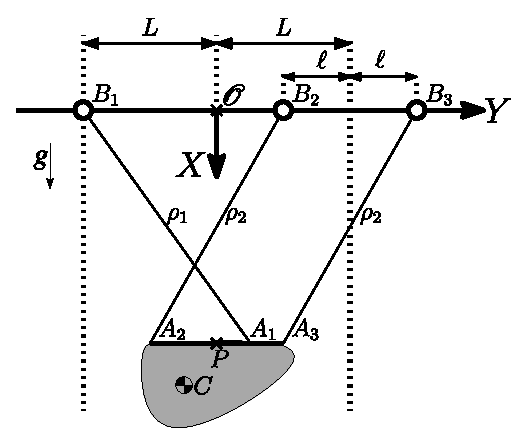
\includegraphics{img/geo_base.eps}}
\caption[Mécanisme plan à 2DDL proposé]{\label{fig:chap1:geometrie}Mécanisme parallèle plan à câbles suspendu utilisant un arrangement de câbles en parallélogramme.}
\end{figure}
La géométrie de ce mécanisme est particulièrement intéressante, puisqu'elle permet de contraindre pleinement le mécanisme dans un plan avec seulement 2 moteurs lorsque les câbles sont maintenus sous tension. Effectivement, puisque la largeur de l'effecteur est égale à la distance séparant les poulies en $A_2$ et $A_3$, il existe seulement deux configurations permettant de raccorder les câbles à l'effectuer tout en maintenant les câbles en tension. La première est celle qui résulte en un arrangement des câbles en parallélogramme. La seconde est celle qui résulte en un arrangement des câbles en trapèze isocèle. Cette seconde configuration est présentée à l'annexe A, mais n'est plus considéré pour la suite de l'analyse, car elle nécessite de changer l'orientation de l'effecteur en fonction de la position de celui-ci dans le plan. La configuration en parallélogramme quant à elle permet à l'effecteur de garder une orientation constante dans le plan peut importe sa position. \par
La représentation géométrique du mécanisme de la figure \ref{fig:chap1:geometrie} semble indiquer que le câble reliant $B_1$ à $A_1$ pourrait interférer avec le câble reliant $B_2$ à $A_2$. Cependant, le croisement de ces câbles est la conséquence de la projection du mécanisme sur le plan $XY$. Un prototype de ce mécanisme utiliserait une paire de câbles en parallélogramme pour relier $B_1$ à $A_1$.

\section{Degré de mobilité du mécanisme}
Le degré de mobilité du mécanisme désigne le degré de liberté de la chaîne cinématique constituant le mécanisme [mettre reference Élément de robotique]. Le critère de mobilité général de Tchebychev-Grübler-Kutzbach permet de déterminer le degré de mobilité d'un mécanisme à l'aide de la formule
\begin{align}
\ell = d\left(n-g-1\right) + \sum_{i=1}^g f_i
\end{align}
où $\ell$ est le degré de liberté de la chaîne cinématique, $d$ est la dimension du système de mouvement considéré ($d = 3$ dans un plan), $n$ est le nombre de corps rigides dans la chaîne, $g$ est le nombre d'articulations et $f_i$ est le nombre de degrés de liberté permis par la $i$-ème articulation. Pour utiliser ce critère, il est primordiale de considérer que les câbles du robot sont sous tension. Chaque câbles peut alors être simplifié comme étant un manipulateur de type RPR, ç.-à-d., un joint rotoïde à la base, suivi d'un joint prismatique qui représente la variation de longueur du câble, et un autre joint rotoïde à l'effecteur. La représentation en graphe du mécanisme résultant de cette simplification est présenté à la figure \ref{fig:chap1:graphe_mauvais}, où les cercles représentes des corps rigides et les lignes des articulations. Le corps rigide $B$ est la base, les corps $C_{ij}$ sont les corps associées au câble $i$(chaque câble est représenté par deux corps séparés d'un joint prismatique). En calculant directement le degré de mobilité, on trouve avec la figure \ref{fig:chap1:graphe_mauvais} les valeurs: $n = 8$, $g = 9$, et $f_i=1 \ \forall i$ pour un résultat de $\ell=3$.\par Cette valeur est erronée puisqu'elle ne tient pas compte de l'architecture spéciale des câbles arrangés en parallélogramme. En effet, comme mentionné précédemment, cette architecture empêche la rotation et actionne les câbles formant le parallélogramme de la même façon. Par conséquent deux modifications doivent être apportées au graphe de la figure \ref{fig:chap1:graphe_mauvais} afin de bien représenter le mécanisme. D'abord, les deux manipulateurs $RPR$ représentant les deux câbles parallèles doivent être représenté comme un seul manipulateur puisqu'ils sont actionnés par un seul moteur. Ensuite, Puisque l'orientation de l'effectuer demeure constante en raison de l'architecture des câbles arrangés en parallélogramme, le dernier joint $R$ du manipulateur $RPR$ indépendant doit être enlevé car un effecteur sans liberté de rotation, dans un graphe est équivalent à un effecteur ponctuel (il n'est pas possible d'avoir deux joints rotoïdes indépendants sur un effecteur ponctuel). La représentation en graphe du mécanisme est alors donnée par la figure \ref{fig:chap1:graphe_bon}. On trouve alors les valeurs $n=5$,$g=5$,$f_i=1\ \forall i$ pour un résultat de $l=2$.
\begin{figure}[t]
\centering
\psfrag{B}[cc][cc][2][0]{$B$}
\psfrag{R}[cc][cc][2][0]{$R$}
\psfrag{P}[cc][cc][2][0]{$P$}
\psfrag{E}[cc][cc][2][0]{$E$}
\resizebox{0.3\textwidth}{!}{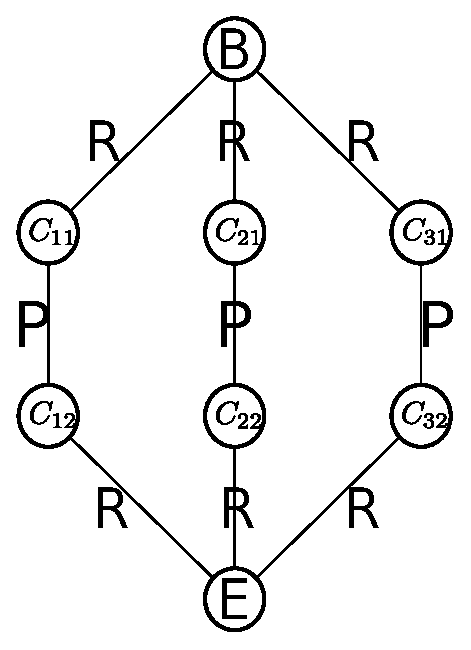
\includegraphics{img/graphes_mauvais.eps}}
\caption{\label{fig:chap1:graphe_mauvais}Graphe d'une mécanisme parallèle avec trois branches $RPR$.}
\end{figure}
\begin{figure}[t]
\centering
\psfrag{B}[cc][cc][2][0]{$B$}
\psfrag{R}[cc][cc][2][0]{$R$}
\psfrag{P}[cc][cc][2][0]{$P$}
\psfrag{C11}[cc][cc][1.5][0]{$C_{11}$}
\psfrag{C12}[cc][cc][1.5][0]{$C_{12}$}
\psfrag{Cm1}[cc][cc][1.5][0]{$C_{m1}$}
\psfrag{Cm2}[cc][cc][1.5][0]{$C_{m2}$}
\resizebox{0.3\textwidth}{!}{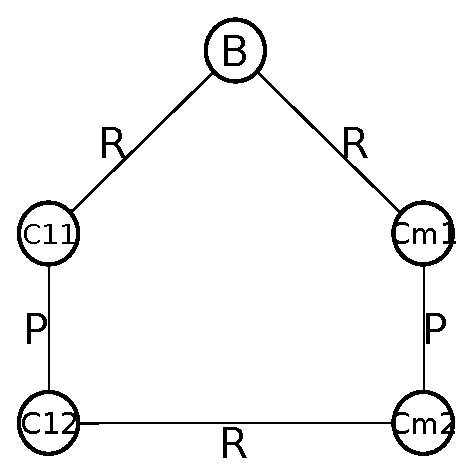
\includegraphics{img/graphe_bon.eps}}
\caption{\label{fig:chap1:graphe_bon}Graphe équivalent au mécanisme parallèle plan.}
\end{figure}
\section{Modélisation cinématique du mécanisme}
Afin de bien mettre en place les nombreuses étapes de la modélisation cinématique, il est important d'expliquer la signification de l'ensemble des variables présentées à la figure \ref{fig:chap1:geometrie} ainsi que d'en présenter d'autres.\\
D'abord, un référentiel fixe, $\mathcal{O}$ est situé sur la base où sont fixées les poulies actionnées. l'axe des $Y$ du référentiel est colinéaire avec la base et croise les trois poulies en leur centre en pointant vers la droite. L'axe de $X$ pointe verticalement vers le bas dans le même sens que la gravité ($g$). L'origine du référentiel fixe est situé à une distance constante $L$ de la poulie en $B_1$. Le vecteur définissant la position de la poulie en $B_1$ est alors $\mathbf{b}_1=\left[0,-L\right]^T$. L'origine est également situé à une distance constante $L$ du point milieu entre les deux poulies en $B_2$ et $B_3$ formant le parallélogramme. La distance séparant les poulies en $B_2$ et $B_3$ est définie comme étant $2\ell$. Les vecteurs donnant les positions constantes des poulies en $B_2$ et $B_3$ sont donc respectivement $\mathbf{b}_2=\left[0,L-\ell\right]^T$ et $\mathbf{b}_3=\left[0,L+\ell\right]^T$. La position de l'effecteur est donnée par le point $P$ qui se situe à distance égale des points d'attache $A_2$ et $A_3$ sur l'effecteur. Il s'agit du point donnant la position de l'effecteur, et donc le vecteur partant de l'origine et point au point $P$ est donné par $\mathbf{p}=\left[x,y\right]^T$. Les vecteurs constants donnant la position des points d'attache $A_2$ et $A_3$ relativement au point $P$ exprimés dans le référentiel de $\mathcal{O}$ sont respectivement $\mathbf{a}_2 = [-\ell,0]^T$ et $\mathbf{a}_3 = [\ell,0]^T$. La position du point d'attache en $A_1$ du câble indépendant par rapport au point $P$ exprimé dans le référentiel de $\mathcal{O}$ est donné par $\mathbf{a}_1=\left[0,a_y\right]$. La position du centre de masse de l'effecteur en $C$ relativement au point $P$ exprimé dans le référentiel de $\mathcal{O}$ est donné par le vecteur constant $\mathbf{c}=\left[c_x,c_y\right]^T$. Les vecteurs de position des différents points d'attache et du centre de masse sont tous exprimés de le référentiel de $\mathcal{O}$ puisque l'effecteur garde une orientation constante de sorte qu'il n'est pas nécessaire de définir une matrice de rotation pour représenter l'orientation de l'effecteur. Les longueurs des câbles sont données par $\rho_1$ et $\rho_2$, où $\rho_2$ est la longueur des deux câbles parallèles.
\subsection{Problème Géométrique Inverse (PGI)}
Le PGI permet de déterminer la longueur des câbles du mécanisme en fonction de la position de l'effecteur. Il s'agit donc d'une étape clé afin de pouvoir contrôler le mécanisme. \par
La première étape de résolution du PGI consiste à calculer une expression vectorielle pour les vecteurs partant des points $B_i$ situés sur la base et allant vers leurs points d'attache respectif en $A_i$ sur l'effecteur ($i = 1,2,3$). Cette expression est donnée par   
\begin{align}
\overrightarrow{B_iA_i}=\mathbf{p} + \mathbf{a}_i-\mathbf{b}_i,i=1,2
\end{align}
où $\overrightarrow{B_iA_i}$ est le vecteur partant du point $B_i$ vers le point $A_i$. La valeur pour $i=3$ n'est pas calculée car $\overrightarrow{B_2A_2}=\overrightarrow{B_3A_3}$ en raison du parallélogramme. De l'équation précédente, on obtient ensuite la valeur de $\rho_i$ en calculant la norme de $\overrightarrow{B_iA_i}$ à l'aide de l'expression
\begin{align}
\rho_i = \sqrt[]{\left(\mathbf{p} + \mathbf{a}_i-\mathbf{b}_i\right)^T\left(\mathbf{p} + \mathbf{a}_i-\mathbf{b}_i\right)},i=1,2.
\label{chap1:eq:PGI}
\end{align}
\subsection{Problème Géométrique Directe (PGD)}
Le PGD permet de déterminer la pose de l'effecteur en fonction de la longueur des câbles. Il s'agit d'un problème quadratique à deux équations et deux inconnus qui peut être résolu à l'aide de l'équation (\ref{chap1:eq:PGI}). Le système de deux équations à deux inconnus suivant est obtenue en élevant au carré l'équation (\ref{chap1:eq:PGI}) et en développant la forme scalaire
\begin{align}
x^2+y^2+E_1y+F_1 = 0 \label{chap1:eq:PGD1}\\
x^2+y^2+E_2y+F_2 = 0, \label{chap1:eq:PGD2}
\end{align}
où 
\begin{alignat}{3}
\quad E_1 &= 2(a_y+L),\quad &F_1 &= (a_y+L)^2-\rho_1^2\\
E_2 &= -2L,\quad &F_2 &= L^2-\rho_2^2.
\end{alignat}
En soustrayant à l'équation (\ref{chap1:eq:PGD2}) l'équation (\ref{chap1:eq:PGD1}) et en isolant $y$, l'équation suivante est obtenue
\begin{align}
y = \beta \label{chap1:eq:isol_x}
\end{align}
où 
\begin{align}
\beta = \frac{F_1-F_2}{E_2-E_1}.
\end{align}
En substituant cette l'équation (\ref{chap1:eq:isol_x}) dans l'équation (\ref{chap1:eq:PGD2}), une équation quadratique qui est seulement fonction de $x$ est obtenue. Les deux solution de cette équation sont alors
\begin{align}
x_1 = \sqrt[]{-(\beta^2+E_2\beta+F_2)}\label{chap1:eq:PGD_solx1}\\
x_2 = -\sqrt[]{-(\beta^2+E_2\beta+F_2)}\label{chap1:eq:PGD_solx2}.
\end{align}
Comme l'effecteur du mécanisme doit toujours être sous la base des poulies, seul la solution $x_1$ est valide. 
À l'aide des équations (\ref{chap1:eq:PGD_solx1}) et (\ref{chap1:eq:isol_x}), il est possible de déterminer la position de l'effecteur en fonction de la longueur des câbles. La section suivante présente les équations de vitesse du mécanisme ce qui permettra par la suite de déterminer les lieux de singularité  du mécanisme.
\subsection{Équations de vitesse}
Les équations de vitesse sont obtenues en dérivant les équations en (\ref{chap1:eq:PGI}) mises au carré. La dérivation prend la forme
\begin{align}
\frac{d\rho_i^2}{dt}=\frac{d}{dt}\left(\left(\mathbf{p} + \mathbf{a}_i-\mathbf{b}_i\right)^T\left(\mathbf{p} + \mathbf{a}_i-\mathbf{b}_i\right)\right)\\
\Rightarrow\rho_i\dot{\rho}_i = \left(\mathbf{p} + \mathbf{a}_i-\mathbf{b}_i\right)^T\dot{\mathbf{p}}, i=1,2.
\end{align}
Sous une forme matricielle, Ce système à deux équations prend la forme
\begin{align}
\mathbf{K}\dot{\bm{\theta}}=\mathbf{J}\dot{\mathbf{x}}
\end{align}
où
\begin{align}
\mathbf{K} = \begin{bmatrix}
\rho_1 & 0\\0 & \rho_2
\end{bmatrix},\quad 
\bm{\theta} =\begin{bmatrix}
 \dot{\rho}_1\\
 \dot{\rho}_2
 \end{bmatrix}
 \quad
 \mathbf{J}=
 \begin{bmatrix}
 \left(\mathbf{p} + \mathbf{a}_1-\mathbf{b}_1\right)^T \\
 \left(\mathbf{p} + \mathbf{a}_2-\mathbf{b}_2\right)^T
\end{bmatrix},\quad
\dot{\mathbf{x}}=
\begin{bmatrix}
\dot{x}\\
\dot{y}
\end{bmatrix}
\end{align}
\subsection{Lieux de singularité}
À l'aide des équations de vitesse de la section précédente sous forme matricielle, il est possible de déterminer les lieux de singularité du mécanisme en calculant les déterminants respectifs des matrices $\mathbf{K}$ et $\mathbf{J}$. Les lieux de singularité sont des position de l'effecteur qui sont à éviter car le contrôle du mécanisme, à cette position, est impossible. 
\subsubsection{Singularité de type I}
Ce type de singularité advient lorsque la matrice $\mathbf{K}$ est singulière, c'est-à-dire lorsque $\text{det}(\mathbf{K})=0$. Il est alors possible de produire des vitesses articulaires infinitésimales sans produire de vitesses cartésiennes à l'effecteur. Ce type de singularité advient habituellement à la limite de l'espace de travail statique du mécanisme, c'est-à-dire l'espace dans lequel l'effecteur peut être au repos à n'importe quel point. Pour le présent mécanisme, ce type de singularité advient lorsque
\begin{align}
\rho_1\rho_2=0.
\end{align}
Cette équation nécessite que $\rho_1$, $\rho_2$ ou $\rho_1$ et $\rho_2$ soit égale à 0. L’éventualité que l'une de ces situations adviennent est simplement évité si l'effecteur reste sous la base des poulies. 
\subsubsection{Singularité de type II}
Ce type de singularité advient lorsque la matrice $\mathbf{J}$ est singulière, donc lorsque $\text{det}(\mathbf{J})=0$. Dans cette position, il est alors possible de produire des mouvements infinitésimales à l'effecteur sans changer la position des actionneurs. Pour le mécanisme à l'étude, cette singularité advient lorsque
\begin{align}
2L+a_y=0.
\end{align}
Dans une telle configuration, les trois câbles du mécanisme deviennent parallèles ce qui résulte en la perte de la liberté de mouvement le long de l'axe $Y$ dans la figure \ref{fig:chap1:geometrie}.  

\section{Modélisation dynamique}
La modélisation dynamique permet de mettre en relation les forces agissant sur un corps avec le mouvement de ce corps. Cette modélisation est basée principalement sur les équations de Newton-Euler. Ces équations sont regroupés sous une forme matricielle, et prennent ainsi la forme
\begin{align}
\begin{bmatrix}
\mathbf{F}\\\mathbf{G}
\end{bmatrix} =
\begin{bmatrix}
m\mathbf{I}_k & 0 \\
0 & \mathbf{I}_{cm}
\end{bmatrix}
\begin{bmatrix}
\ddot{\mathbf{p}}\\\bm{\alpha}
\end{bmatrix} + 
\begin{bmatrix}
0 \\
\bm{\omega} \times \mathbf{I}_{cm}\bm{\omega}
\end{bmatrix}, \label{chap1:eq:NEGEN}
\end{align}
où $\mathbf{F}$ est le vecteur de la somme des forces agissants sur le centre de masse du corps, $\mathbf{G}$ est le vecteur de la somme des couples agissants sur le mécanisme, $m$ est la masse du corps, $\mathbf{I}_k$ est une matrice identité de niveau $k$ où $k$ est le nombre de degrés de liberté en translation du corps, $\mathbf{I}_{cm}$ est le torseur d'action des moments d'inertie du corps par rapport à son centre de masse, $\ddot{\mathbf{p}}$ est le vecteur des accélérations du centre de masse de du corps exprimé dans un référentiel inertiel, $\bm{\alpha}$ est le vecteur des accélérations angulaires du corps et $\bm{\omega}$ représente le vecteur des vitesses angulaires du corps. L'application de ces équations à l'effecteur du robot présenté dans ce chapitre requiert que les termes $\bm{\alpha}$ et $\bm{\omega}$ soient nuls afin d'assurer que les câbles parralèles du mécanisme soit toujours en tension. De plus, puisque le robot est planaire, le vecteur $\mathbf{F}$ n'a que deux composantes de sorte que $\mathbf{I}_k$ est une matrice identité de deuxième ordre et le vecteur $\mathbf{G}$ devient un scalaire. L'application de l'équation (\ref{chap1:eq:NEGEN}) à l'effecteur du robot s'écrit alors 
\begin{align}
\begin{bmatrix}
\sum\limits_{i=1}^3\left(-f_i\mathbf{e}_i\right)+m\mathbf{g}\\
\sum\limits_{i=1}^3\left(\mathbf{c}-\mathbf{a}_i\right)^T\mathbf{E}\left(-f_i\mathbf{e}_i\right)
\end{bmatrix} = 
\begin{bmatrix}
m\ddot{\mathbf{p}}\\
0
\end{bmatrix}
\label{chap1:eq:NE}
\end{align} 
où 
\begin{align}
\mathbf{e}_i=\frac{\mathbf{p}+\mathbf{a}_i-\mathbf{b}_i}{\rho_i},i=1,2,3 \label{u_length}
\end{align}
sont des vecteurs unitaires parallèles aux câbles respectif et partant de leur point $B_i$ respectif, où $f_i, i=1,2,3$ représente la tension de la câble $i$ (le câble $i$ désigne le câble partant du point $B_i$ vers le point $A_i$), où $\ddot{\mathbf{p}}$ désigne le vecteur des accélérations exprimé dans le repère de $\mathcal{O}$, où $\mathbf{g}=[g,0]^T$ est le vecteur de l'accélération gravitationnelle et où 
\begin{align}
\mathbf{E}=\begin{bmatrix}
0 & -1\\1 & 0
\end{bmatrix}
\end{align} 
est une matrice permettant de faire des produits croisés dans un plan. \par
L'équation (\ref{chap1:eq:NE}) peut être réécrite sous la forme
\begin{align}
\mathbf{M}\bm{\tau}=\bm{\gamma} \label{mat_n_e},
\end{align}
où
\begin{align} \bm{\gamma} =\begin{bmatrix} \mathbf{g-\ddot{p}}\\0 \end{bmatrix}, \label{gamma} \end{align} \begin{align} \bm{\tau} = \frac{1}{m}\mathbf{f}=\frac{1}{m}\begin{bmatrix} f_1 & f_2 & f_3 \end{bmatrix}^T, \label{tau} \end{align} \begin{align} \mathbf{M}=\begin{bmatrix} \mathbf{e}_1 & \mathbf{e}_2 & \mathbf{e}_3\\
\delta_1 &\delta_2 &    \delta_3 \end{bmatrix},
\label{M}\end{align}
\begin{align}
\delta_i=(\mathbf{a}_i-\mathbf{c})^T\mathbf{E}\mathbf{e}_i,\quad i=1,2,3.\label{alpha}
\end{align}
En (\ref{tau}), $\bm{\tau}$ est un vecteur contenant la tension de chaque câble par unité de masse de l'effecteur ($m$). \par 
L'inversion de la matrice $\mathbf{M}$ dans l'équation (\ref{mat_n_e}) permet d'obtenir des expressions pour les tensions par unité de masse dans les câbles en fonction de l'accélération et la position de l'effecteur. Cette inversion s'écrit
\begin{align}
\bm{\tau}=\mathbf{M}^{-1}\bm{\gamma}.\label{inv_dyn}
\end{align}
Le calcul de la matrice inverse $\mathbf{M}^{-1}$ peut se faire à l'aide de la méthode des cofacteurs qui prend la forme
\begin{align}
\mathbf{M}^{-1} =  \frac{\text{Adj}(\mathbf{M})}{\text{det}(\mathbf{M})}, \label{M_inv}
\end{align}
où $\text{Adj}(\mathbf{M})$ est la comatrice de $\mathbf{M}$ et $\text{det}(\mathbf{M})$ est son déterminant. Cependant, il faut d'abord déterminer si $\mathbf{M}$ n'est pas singulière, c'est-à-dire que 
$\text{det}(\mathbf{M})\neq 0$. Le déterminant de la matrice se calcule \begin{align}
\text{det}(\mathbf{M})=\delta_1(\mathbf{e}_2^T\mathbf{E}\mathbf{e}_3)-\delta_2(\mathbf{e}_1^T\mathbf{E}\mathbf{e}_3)+\delta_3(\mathbf{e}_1^T\mathbf{E}\mathbf{e}_2). \label{chap1:eq:det_M_1}
\end{align}
Or, $\mathbf{e}_2 = \mathbf{e}_3$ puisque les câbles 2 et 3 sont parallèles. Par conséquent, l'équation (\ref{chap1:eq:det_M_1}), après substitutions des $\delta_i$ par leur expressions respectives et remplacement des $\mathbf{e}_3$ par $\mathbf{e}_2$ devient
\begin{align}
\text{det}(\mathbf{M}) = \left(\mathbf{a}_2-\mathbf{a}_3\right)^T\mathbf{E}\mathbf{e}_2\left(\mathbf{e}_1^T\mathbf{E}\mathbf{e}_2\right)\label{chap1:eq:det_M_2}.
\end{align}
Pour que l'expression à la droite de l'égalité (\ref{chap1:eq:det_M_2}) soit égale à 0, il faut que l'une des éventualités suivante se produise:
\begin{enumerate}
\item Si $\mathbf{a}_2 = \mathbf{a}_3$. Cependant, si l'effecteur n'est pas une masse ponctuelle, cette éventualité n'est pas possible.
\item Si $\mathbf{e}_2=0$. Cette éventualité est coïncidente avec la singularité de type I présentée précédemment. Si l'effecteur reste sous la base des poulies, $\mathbf{e}_2$ ne sera jamais égale à 0.
\item Si $\mathbf{e}_1=0$. La même logique que pour le point précédent s'applique.
\item Si $\left(\mathbf{a}_2-\mathbf{a}_3\right)^T\mathbf{E}\mathbf{e}_2=0$. Cela advient lorsque $\left(\mathbf{a}_2-\mathbf{a}_3\right)$ devient colinéaire avec $\mathbf{e}_2$. Le seul endroit où cela se produit est à la hauteur de la base des poulies. Par conséquent, si l'effecteur reste sous la base des poulies, cette éventualité ne devrait pas se produire. 
\item Si $\mathbf{e}_1^T\mathbf{E}\mathbf{e}_2=0$. Pour que cela se produise, il faudrait que $\mathbf{e}_1$ et $\mathbf{e}_2$ deviennent colinéaire. Par conséquent, si l'effecteur demeure sous la base des poulies, cette éventualité n'adviendra jamais.  
\end{enumerate}
Plusieurs des éventualités dans la liste précédente sont coïncidente avec la situation où l'effecteur est à la hauteur de la base des poulies. Or, si l'effecteur demeure sous cette base, le signe des termes composants le déterminant de la matrice $\mathbf{M}$ demeure constant peut importe la position sous la base des poulies. En effet, $\left(\mathbf{a}_2-\mathbf{a}_3\right)^T\mathbf{E}\mathbf{e}_2$ est toujours positif tandis que $\mathbf{e}_1^T\mathbf{E}\mathbf{e}_2=0$ est toujours négatif. Par conséquent, $\text{det}(\mathbf{M})$ est toujours négatif.
\par 
Afin d'assurer le bon contrôle du mécanisme, il est nécessaire de toujours avoir de la tension dans les câbles peut importe la position de l'effecteur. Mathématiquement, cette condition s'écrit
\begin{align}
\bm{\tau} \succ \mathbf{0},
\end{align}
où $\succ$ désigne l'inégalité pour chaque composante de $\bm{\tau}$. Considérant cette condition, l'équation (\ref{inv_dyn}) et le fait que $\text{det}(\mathbf{M})<0$ lorsque l'effecteur se situe sous la base des poulies, il est possible d'écrire une condition mathématique vectorielle en fonction de la position et l'accélération de l'effecteur qui assure que les câbles du mécanisme sont toujours en tension peut importe la position de l'effecteur. Cette condition prend la forme
\begin{align} \text{Adj}(\mathbf{M})\bm{\gamma}\prec \mathbf{0}.\label{cond_ten_2} \end{align}
La comatrice $\text{Adj}(\mathbf{M})$ se calcule alors comme 
\begin{align}
\text{Adj}(\mathbf{M})=\begin{bmatrix}
\bm{\epsilon}_1^T\\
\bm{\epsilon}_2^T\\
\bm{\epsilon}_3^T
\end{bmatrix}
\label{adj_m}
\end{align}
où
\begin{align}
\bm{\epsilon}_1=\begin{bmatrix}
\mathbf{e}_2\\\delta_2
\end{bmatrix}\times \begin{bmatrix}
\mathbf{e}_2\\\delta_3
\end{bmatrix},
\label{epsi1}\\
\bm{\epsilon}_2=\begin{bmatrix}
\mathbf{e}_2\\\delta_3
\end{bmatrix}\times \begin{bmatrix}
\mathbf{e}_1\\\delta_1
\end{bmatrix},
\label{epsi2}\\
\bm{\epsilon}_3=\begin{bmatrix}
\mathbf{e}_1\\\delta_1
\end{bmatrix}\times \begin{bmatrix}
\mathbf{e}_2\\\delta_2
\end{bmatrix}.
\label{epsi3}
\end{align}
La forme scalaire de (\ref{cond_ten_2}) est un système de 3 inégalités différentielles qui s'écrit
\begin{align}
\left(g-\ddot{x}\right)(A_i+B_iy) +\ddot{y}(C_i+B_ix)<0,\quad i=1,2,3, \label{cond_scal}
\end{align}
où
\begin{alignat*}{6}
&A_1 &&= -L,\quad &&A_2 &&= a_y(c_y-L)+2Lc_y-\ell(a_y+L) , \quad &&A_3 &&= a_y(L-cy)-2Lc_y-\ell(a_y+L),\\
&B_1 &&= 1,\quad &&B_2 &&= a_y-\ell,\quad &&B_3 &&= -(a_y+\ell),\\
&C_1 &&= 0,\quad &&C_2 &&= c_x(2L+a_y),\quad &&C_3 &&= -C_2.
\end{alignat*}
Lorsque ces inégalités sont toutes satisfaites, la tension dans les câbles est assurée. Ces inégalités sont donc les critères principaux pour déterminer s'il est possible d'entreprendre une certaine trajectoire ou encore s'il est possible de rester au repos à une certaine position. La section suivante utilise les inégalités en (\ref{cond_scal}) afin de déterminer l'ensemble des positions du centre de masse où l'effecteur peut être maintenue au repos.
\section{Espace de travail statique}
Le respect des inégalités en (\ref{cond_scal}) permet d'assurer la tension dans les câbles du mécanisme en considérant la position et les accélération de l'effecteur. Ces inégalités permettent également de définir l'espace de travail statique du mécanisme. Cet espace est ici définie comme l'ensemble des positions du point $P$ où l'effecteur peut être au repos par rapport au référentiel inertiel (dans le cas présent, $\mathcal{O}$) sans subir d'accélérations autres que l'accélération gravitationnelle. Pour obtenir les inégalités qui permettent de définir l'espace statique de travail en fonction des inégalités en (\ref{cond_scal}), il faut alors poser $\ddot{x}=\ddot{y}=0$. Les inégalités deviennent alors
\begin{align}
A_i+B_iy <0, i=1,2,3. \label{chap1:ineq:ES1}
\end{align}
En isolant $y$ dans les inégalités en (\ref{chap1:ineq:ES1}), un intervalle fermé est obtenue qui délimite l'espace statique de travail le long de l'axe $Y$ du référentiel $\mathcal{O}$. Cet intervalle s'écrit
\begin{align}
y \in \left]\max\left(-\frac{A_2}{B_2},-\frac{A_3}{B_3}\right),L\right[.\label{dom_stat}
\end{align}
où max() est une fonction qui retourne la valeur maximale de ses arguments. Comme mentionné précédemment, le point $A_1$ est situé entre les points $A_2$ et $A_3$ dans le cadre de cette étude. Cela implique alors que le paramètre $a_y$ est limité à l'intervalle $a_y \in \left]-\ell,\ell\right[$. Cette limitation du paramètre $a_y$ implique également une limitation du paramètre $c_y$ à l'intervalle $\left]-\ell,\ell\right[$. En effet, si le point $A_1$ se situe entre les points $A_2$ et $A_3$, alors le centre de masse doit également se situer entre les point $A_2$ et $A_3$ car sinon, les moments appliqués par chaque câble atour du centre de masse seraient tous de même direction ce qui empêcherait l'effecteur d'avoir une orientation constante. Ce choix arbitraire permet de contraindre l'analyse de l'influence du paramètre $a_y$ à un intervalle fermé plutôt que ouvert. L'annexe B présente une courte analyse de l'espace statique de travail lorsque le paramètre $a_y$ n'est pas limité à un intervalle. \par 
La borne supérieure de l'espace de travail est toujours coïncidente avec la position $y = L$ car il s'agit du point où les deux câbles parallèles sont verticaux. À ce moment, l'ensemble du poids de l'effecteur est supporté par ces deux câbles tandis qu'aucune tension n'est présente dans le câble indépendant. La borne inférieure de l'intervalle en (\ref{dom_stat}) est coïncidente avec la position en $y$ où l'un des deux câbles parallèle perd complètement sa tension. La fonction max() permet ainsi de distinguer lequel des deux câbles sera flasque en premier et délimitera donc en premier l'espace de travail statique.\par
Afin de bien visualiser la relation entre l'intervalle (\ref{dom_stat}) et la tension dans les câbles du mécanisme, la figure \ref{chap1:fig:ten_stat} présente l'évolution de la tension dans les câbles en fonction de la position en $y$ de l'effecteur.
\begin{figure}[h!]
\centering
\psfrag{s01}[cc][cc][1.2][0]{$y/L$ \ [m/m]}
\psfrag{s02}[cc][cc][1.2][0]{$f_i/mg$ \ [N/N]}
\psfrag{f1}{$f_1$}
\psfrag{f2}{$f_2$}
\psfrag{f3}{$f_3$}
\psfrag{f12}{$y_{\text{min}}$}
\psfrag{f32}{$y_{\text{max}}$}
\psfrag{yeq}[cl][cc][1.2][0]{$\leftarrow\text{max}\left(-\frac{A_2}{B_2},-\frac{A_3}{B_3}\right)$}
\psfrag{title}[cc][cc][1][0]{$L=5$ m, $\ell = 1$ m, $a_y =0.4$ m, $c_x = 0.1$ m, $c_y =-0.1$ m }
\resizebox{0.75\textwidth}{!}{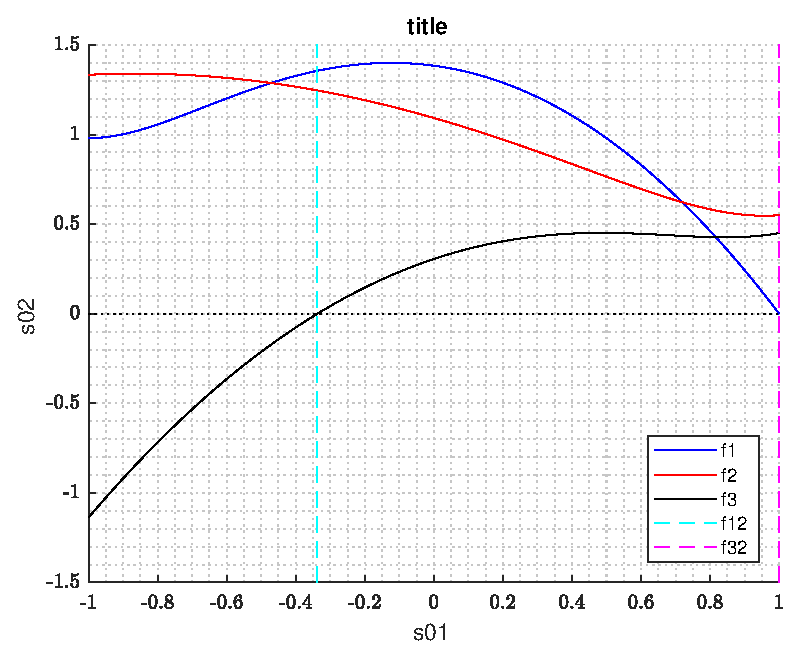
\includegraphics{img/espace_stat_tension.eps}}
\caption{\label{chap1:fig:ten_stat} Tension dans les câbles en fonction de la position statique en $y$.}
\end{figure}
L'abscisse de la figure présente la position de l'effecteur en $y$ divisé par $L$. Ce rapport permet de faire abstraction de l'ordre de grandeur de l'espace de travail en $y$. Les ordonnés représentent l'évolution de la tension dans les câbles divisé par le poids de l'effecteur, $mg$. Cette quantité est renommée tension relative pour faciliter l'écriture. Les courbes pleines bleue, rouge et noire représentent respectivement les tensions relatives dans les câbles 1,2 et 3. La ligne en trait discontinu magenta, $y_{max}$ désigne la borne supérieure de l'intervalle en (\ref{dom_stat}). La ligne en trait discontinu cyan, $y_{min}$, représente, quant à elle, la borne inférieure. Les valeurs des paramètres géométriques du mécanisme ($L,\ell,a_y,c_x,c_y$) sont tous définis dans le haut de la figure. \par
La ligne $y_{min}$ croise la ligne de tension nulle en pointillée à la même position que la courbe montrant la tension relative du câble 3. Dans cette configuration du mécanisme, le câble 3 est donc celui qui limite l'espace statique de travail. La ligne $y_{max}$ croise la ligne de tension nulle au point $y=L$, ce qui est coïncident avec l'intersection entre la courbe de tension relative du câble 1 avec la ligne de tension nulle. Par conséquent, à cette position, c'est le câble 1 qui limite l'espace de travail statique.\par
Le paramètre $c_x$ n'a aucune influence sur l'espace statique de travail. Cela est dû au fait que la distance entre chaque point d'attache $A_i, i=1,2,3$ et le centre de masse $C$ projetée sur l'axe $X$ est égale. Par conséquent, chaque «levier» de moment le long de l'axe $X$ est équivalent, et l'équilibre, pour cette composante du moment, est simplement conservée si la somme des forces, projetée sur l'axe des $Y$, est égale à 0. Il s'agit d'une propriété très intéressante pour des applications de transport puisque le soulèvement de charge change la position du centre de masse, mais si le centre de masse de la charge est placée directement sous le centre de masse de l'effecteur, alors la masse de la charge soulevé n'aura aucune influence sur l'espace de travail statique. \par
L'espace de travail statique qui est défini à l'équation (\ref{dom_stat}) n'est également pas fonction de la variable $x$, qui indique la position de l'effecteur selon l'axe $X$. Cela est dû au fait que toutes les valeurs de $x>0$ sont inclues dans l'espace statique de travail puisque la gravité pointe dans la même direction que l'axe $X$.
\subsubsection{Largeur de l'espace de travail statique}
D'après l'intervalle en (\ref{dom_stat}) définissant l'espace statique le long de l'axe $Y$, la largeur de l'espace de travail statique $\mathcal{L}$ s'écrit
\begin{align}
\mathcal{L} = L - \text{max}\left(-\frac{A_2}{B_2},-\frac{A_3}{B_3}\right).
\label{chap1:eq:larg:stat}
\end{align}
Dans l'équation (\ref{chap1:eq:larg:stat}), $\mathcal{L}$ est fonction des paramètres $L,\ell,a_y$ et $c_y$. De ces paramètres, seulement les paramètres $\ell$ et $a_y$ sont ici jugés comme des paramètres contrôlables. En effet, le paramètre $L$ est en réalité un indicateur de l'ordre de grandeur du mécanisme et est fonction de l'utilisation du robot. Le paramètre $c_y$ est, quant à lui, une quantité qui peut varier en fonction de la masse et de la forme de l'effecteur et de l'object qui est soulevé par le robot. L'optimisation de l'espace de travail maximale est donc obtenue déterminant les valeurs de $a_y$ et $\ell$ qui maximisent $\mathcal{L}$ dans l'équation (\ref{chap1:eq:larg:stat}). \par 
La première étape pour obtenir ces valeurs consiste à calculer le gradiant de $\mathcal{L}$ dans l'espace des paramètres $a_y$ et $\ell$ et de mettre ce gradiant égale à $\mathbf{0}$, où $\mathbf{0}$ est le vecteur nul. En faisant ceci, les extrêmes de $\mathcal{L}$ seront obtenus. Mathématiquement, cela s'écrit
\begin{align}
\bm{\nabla} \mathcal{L} = \mathbf{0},
\end{align}
où $\bm{\nabla}$ est l'opérateur du gradiant dans l'espace des paramètres $a_y$ et $\ell$ et est donc écrit comme 
\begin{align}
\bm{\nabla} = 
\begin{bmatrix}
\frac{\partial }{\partial a_y}\\
\frac{\partial }{\partial \ell}
\end{bmatrix}.
\end{align}
L'équation en (\ref{chap1:eq:larg:stat}) est difficilement différentiable en raison de la fonction max(). Cependant, il est possible de faire du cas par cas. Le cas A est ici défini comme le moment où $-\frac{A_2}{B_2}>-\frac{A_3}{B_3}$, et le cas B est défini comme le moment où $-\frac{A_2}{B_2}<-\frac{A_3}{B_3}$. \par
\subsubsection{cas A}
le gradiant se calcule
\begin{align}
\bm{\nabla} \mathcal{L} =
\begin{bmatrix}
\frac{\partial }{\partial a_y}\\
\frac{\partial }{\partial \ell}
\end{bmatrix}\frac{LB_2+A_2}{B_2} = \begin{bmatrix}
\frac{(2L+\ell)(\ell-c_y)}{(a_y-l)^2}\\
\frac{(2L+a_y)(c_y-a_y)}{(a_y-l)^2}
\end{bmatrix}.
\end{align}
La seule solution logique du système d'équation $\bm{\nabla} \mathcal{L} = \mathbf{0}$ pour les valeurs $a_y$ et $l$ est alors 
\begin{align}
a_y = \ell = c_y.
\end{align}
En entrant ces valeurs dans l'équation (\ref{chap1:eq:larg:stat}), la valeur suivante est obtenue
\begin{align}
\mathcal{L} = L+\ell. 
\end{align}
Cette valeur est un maximum de la fonction en (\ref{chap1:eq:larg:stat}). Ce résultat aurait pu être déduit par simple inspection de la figure \ref{fig:chap1:geometrie}. En effet, lorsque la condition $a_y = \ell = c_y$ est satisfaite, le robot devient équivalent à un robot à masse ponctuelle avec seulement deux câbles, les câbles 1 et 3. La figure \ref{chap1:fig:compare_pm} suivante présente le mécanisme dans cette condition en métant en évidence le robot équivalent à deux câbles. Dans cette condition, les vecteurs de tension dans les câbles 1 et 3 passent par le centre de masse de sorte qu'il n'appliquent aucun moment sur le centre de masse. De plus, puisque la force de poids de l'effecteur passe également par le centre de masse, la tension dans le câble 2 est obligatoirement nulle afin de conserver l'orientation constante de l'effecteur. 
\begin{figure}[h]
\centering
\resizebox{0.75\textwidth}{!}{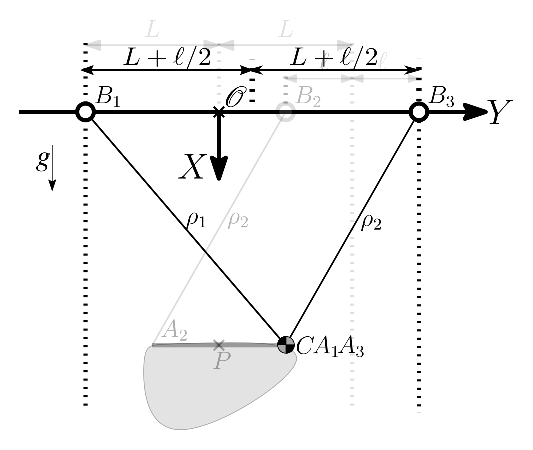
\includegraphics{img/geo_base_comp_pm.eps}}
\caption{\label{chap1:fig:compare_pm} Disposition géométrique maximisant la largeur de l'espace de travail statique.}
\end{figure}
\subsubsection{cas B}
En appliquant la même méthode que pour le cas A, la solution du système d'équation $\bm{\nabla} \mathcal{L} = \mathbf{0}$ pour les valeurs $a_y$ et $\ell$ dans le cas B est 
\begin{align}
c_y = -\ell, a_y =\ell.
\end{align}
En entrant ces valeurs dans l'équation (\ref{chap1:eq:larg:stat}) dans le cas B, la valeur suivante est obtenue
\begin{align}
\mathcal{L} = 0. 
\end{align}
Cette valeur est la valeur minium de la fonction en (\ref{chap1:eq:larg:stat}). Ce résultat aurait également pu être déduit par inspection de la figure \ref{fig:chap1:geometrie}. Lorsque $-a_y=c_y=-\ell$, le robot devient équivalent à un pendule qui est suspendue seulement au câble 2. La figure \ref{chap1:fig:compare_pm_min} présente le robot dans cette configuration en métant en évidence le pendule. Dans cette condition, les câbles 1 et 3 appliquent leur tension à partir du même point sur l'effecteur du robot et on, par conséquent, le même levier. À toutes les positions sous la base des poulies, ces câbles appliquent donc des moment dans la même direction. Or, le câble 2 n'applique aucun moment sur l'effecteur puisque son point d'attache est coïncident avec le centre de masse de l'effecteur. La tension dans les câbles 1 et 3 n'a alors d'autre que choix que d'être nulle afin de conserver l'orientation constante de l'effecteur. Cependant, puisque seul le câble 2 est en tension, celui-ci est nécessairement vertical afin de conserver un équilibre statique (aucune autre force n'est appliquée sur l'effecteur dans l'axe des $Y$). Comme il s'agit de la seule configuration possible pour le robot dans cette condition, la largeur de l'espace statique est alors nulle.\par
\begin{figure}[h] 
\centering
\resizebox{0.75\textwidth}{!}{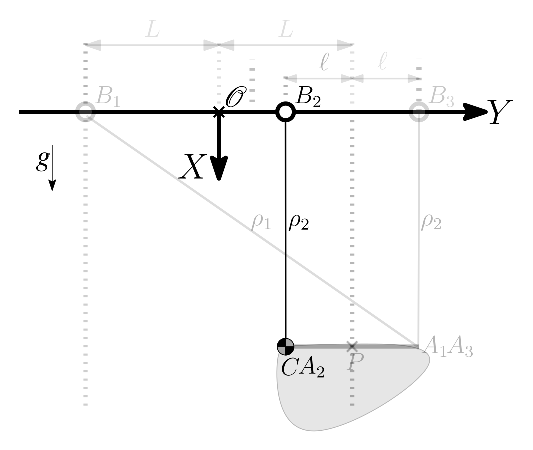
\includegraphics{img/geo_base_comp_pm_min.eps}}
\caption{\label{chap1:fig:compare_pm_min} Disposition géométrique minimisant la largeur de l'espace de travail statique.}
\end{figure}
Les deux cas précédent montre des arrangements géométriques extrêmes de l'effecteur. Or, il existe une quantité infinie d'arrangement différents qui offre une largeur de l'espace de travail statique $\mathcal{L}$ plus ou moins grande. Les figures en \ref{chap1:fig:stat_max} présentent la variation de $\mathcal{L}$ en fonction des paramètres $a_y$ et $c_y$ variant de $-\ell$ à $\ell$ pour différentes valeurs de $\ell$. \clearpage
\begin{figure}[h!]
\centering
\begin{subfigure}[h]{0.8\textwidth}
\psfrag{-0.1}[cc][cc][1][0]{$0.1$}
\psfrag{-0.2}[cc][cc][1][0]{$0.2$}
\psfrag{-0.3}[cc][cc][1][0]{$0.3$}
\psfrag{-0.4}[cc][cc][1][0]{$0.4$}
\psfrag{-0.5}[cc][cc][1][0]{$0.5$}
\psfrag{-0.6}[cc][cc][1][0]{$0.6$}
\psfrag{-0.7}[cc][cc][1][0]{$0.7$}
\psfrag{-0.8}[cc][cc][1][0]{$0.8$}
\psfrag{-0.9}[cc][cc][1][0]{$0.9$}
\psfrag{-1}[cc][cc][1][0]{$-1$}
\psfrag{1}[cc][cc][1][0]{$1$}
\psfrag{0.1}[cc][cc][1][0]{$0.1$}
\psfrag{0.2}[cc][cc][1][0]{$0.2$}
\psfrag{0.3}[cc][cc][1][0]{$0.3$}
\psfrag{0.4}[cc][cc][1][0]{$0.4$}
\psfrag{0.5}[cc][cc][1][0]{$0.5$}
\psfrag{0.6}[cc][cc][1][0]{$0.6$}
\psfrag{0.7}[cc][cc][1][0]{$0.7$}
\psfrag{0.8}[cc][cc][1][0]{$0.8$}
\psfrag{0.9}[cc][cc][1][0]{$0.9$}
\psfrag{0}[cc][cc][1][0]{$0$}
\psfrag{cy-1}[cc][cc][1.2][0]{$c_y/\ell$ \ [m/m]}
\psfrag{ay-1}[cc][cc][1.2][0]{$a_y/\ell$ \ [m/m]}
\psfrag{Ltitle-1}[cc][cc][1.2][0]{$\mathcal{L}/(2L+\ell)$\ [m/m],\quad $\ell/L =0.25$}
\resizebox{1\textwidth}{!}{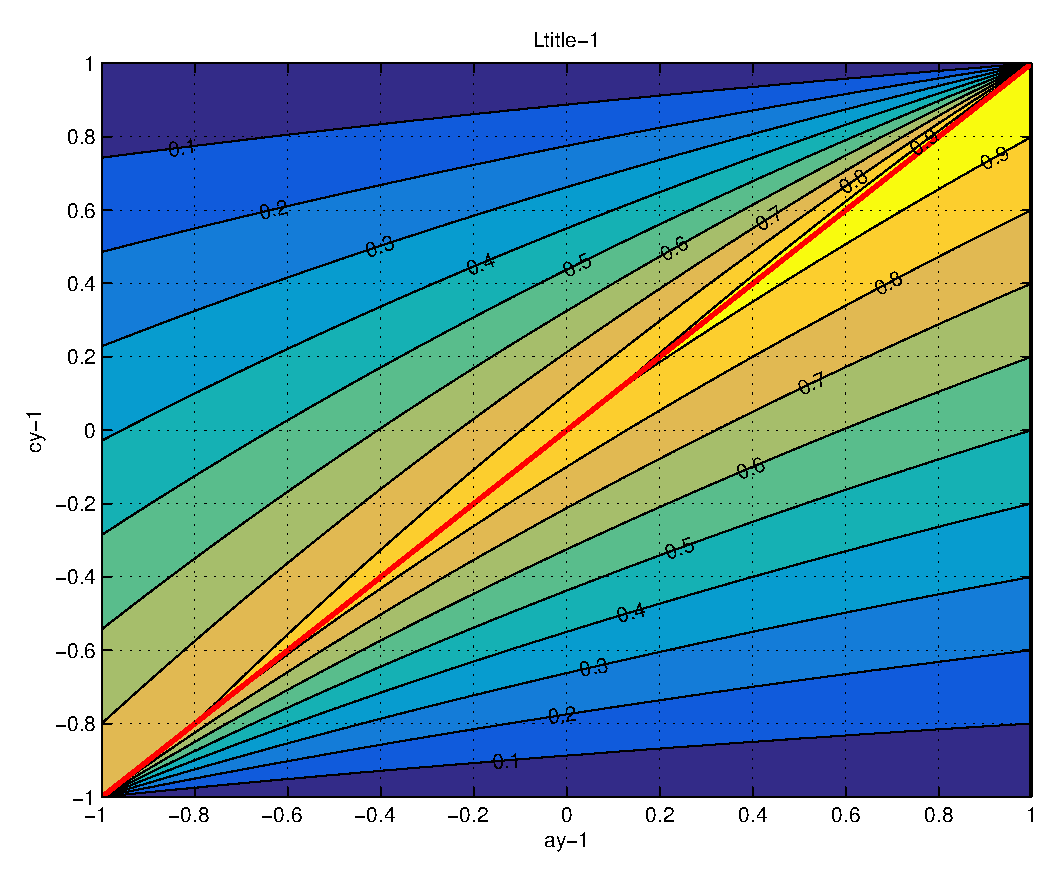
\includegraphics{img/espace_stat_max1.eps}}
\caption{}
\end{subfigure}

\begin{subfigure}[h]{0.8\textwidth}
\psfrag{-0.1}[cc][cc][1][0]{$0.1$}
\psfrag{-0.2}[cc][cc][1][0]{$0.2$}
\psfrag{-0.3}[cc][cc][1][0]{$0.3$}
\psfrag{-0.4}[cc][cc][1][0]{$0.4$}
\psfrag{-0.5}[cc][cc][1][0]{$0.5$}
\psfrag{-0.6}[cc][cc][1][0]{$0.6$}
\psfrag{-0.7}[cc][cc][1][0]{$0.7$}
\psfrag{-0.8}[cc][cc][1][0]{$0.8$}
\psfrag{-0.9}[cc][cc][1][0]{$0.9$}
\psfrag{-1}[cc][cc][1][0]{$-1$}
\psfrag{1}[cc][cc][1][0]{$1$}
\psfrag{0.1}[cc][cc][1][0]{$0.1$}
\psfrag{0.2}[cc][cc][1][0]{$0.2$}
\psfrag{0.3}[cc][cc][1][0]{$0.3$}
\psfrag{0.4}[cc][cc][1][0]{$0.4$}
\psfrag{0.5}[cc][cc][1][0]{$0.5$}
\psfrag{0.6}[cc][cc][1][0]{$0.6$}
\psfrag{0.7}[cc][cc][1][0]{$0.7$}
\psfrag{0.8}[cc][cc][1][0]{$0.8$}
\psfrag{0.9}[cc][cc][1][0]{$0.9$}
\psfrag{0}[cc][cc][1][0]{$0$}
\psfrag{cy-2}[cc][cc][1.2][0]{$c_y/\ell$ \ [m/m]}
\psfrag{ay-2}[cc][cc][1.2][0]{$a_y/\ell$ \ [m/m]}
\psfrag{Ltitle-2}[cc][cc][1.2][0]{$\mathcal{L}/(2L+\ell)$\ [m/m],\quad $\ell/L =0.5$}
\resizebox{1\textwidth}{!}{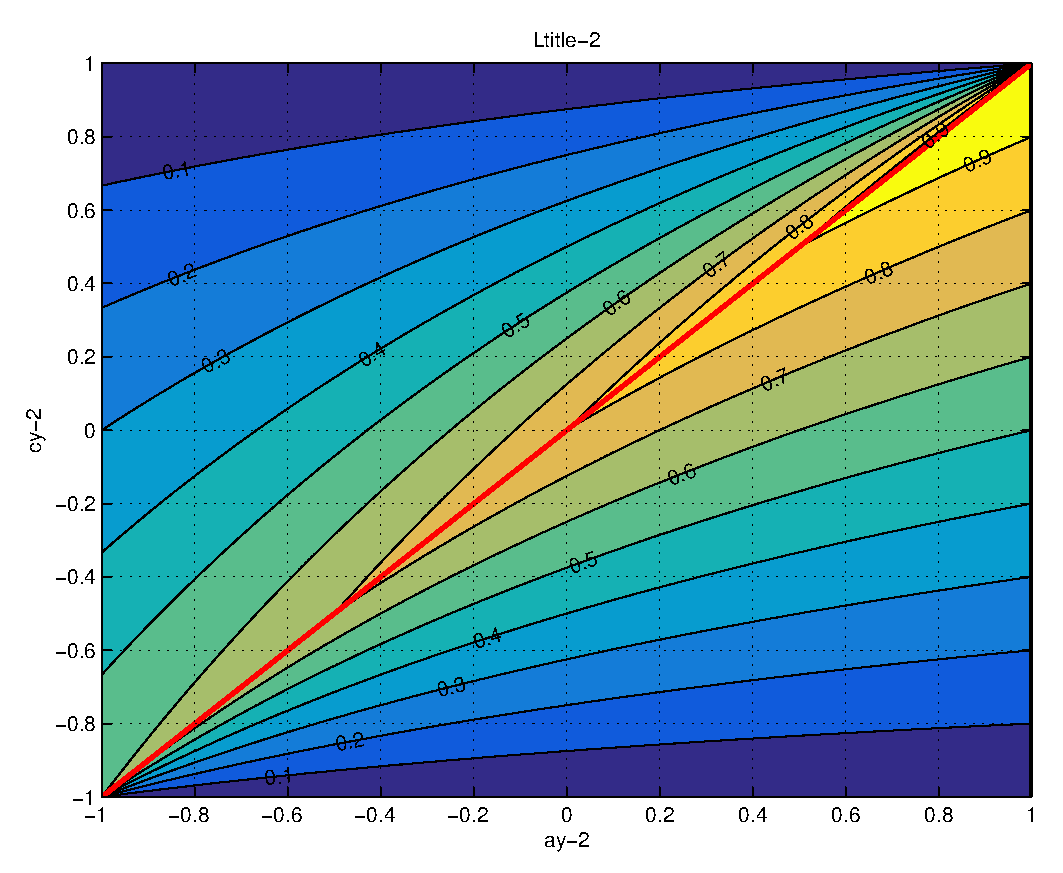
\includegraphics{img/espace_stat_max2.eps}}
\caption{}
\end{subfigure}
\end{figure}
\begin{figure}[h!]\ContinuedFloat
\centering
\begin{subfigure}[h]{0.8\textwidth}
\psfrag{-0.1}[cc][cc][1][0]{$0.1$}
\psfrag{-0.2}[cc][cc][1][0]{$0.2$}
\psfrag{-0.3}[cc][cc][1][0]{$0.3$}
\psfrag{-0.4}[cc][cc][1][0]{$0.4$}
\psfrag{-0.5}[cc][cc][1][0]{$0.5$}
\psfrag{-0.6}[cc][cc][1][0]{$0.6$}
\psfrag{-0.7}[cc][cc][1][0]{$0.7$}
\psfrag{-0.8}[cc][cc][1][0]{$0.8$}
\psfrag{-0.9}[cc][cc][1][0]{$0.9$}
\psfrag{-1}[cc][cc][1][0]{$-1$}
\psfrag{1}[cc][cc][1][0]{$1$}
\psfrag{0.1}[cc][cc][1][0]{$0.1$}
\psfrag{0.2}[cc][cc][1][0]{$0.2$}
\psfrag{0.3}[cc][cc][1][0]{$0.3$}
\psfrag{0.4}[cc][cc][1][0]{$0.4$}
\psfrag{0.5}[cc][cc][1][0]{$0.5$}
\psfrag{0.6}[cc][cc][1][0]{$0.6$}
\psfrag{0.7}[cc][cc][1][0]{$0.7$}
\psfrag{0.8}[cc][cc][1][0]{$0.8$}
\psfrag{0.9}[cc][cc][1][0]{$0.9$}
\psfrag{0}[cc][cc][1][0]{$0$}
\psfrag{cy-3}[cc][cc][1.2][0]{$c_y/\ell$ \ [m/m]}
\psfrag{ay-3}[cc][cc][1.2][0]{$a_y/\ell$ \ [m/m]}
\psfrag{Ltitle-3}[cc][cc][1.2][0]{$\mathcal{L}/(2L+\ell)$\ [m/m],\quad $\ell/L =0.75$}
\resizebox{1\textwidth}{!}{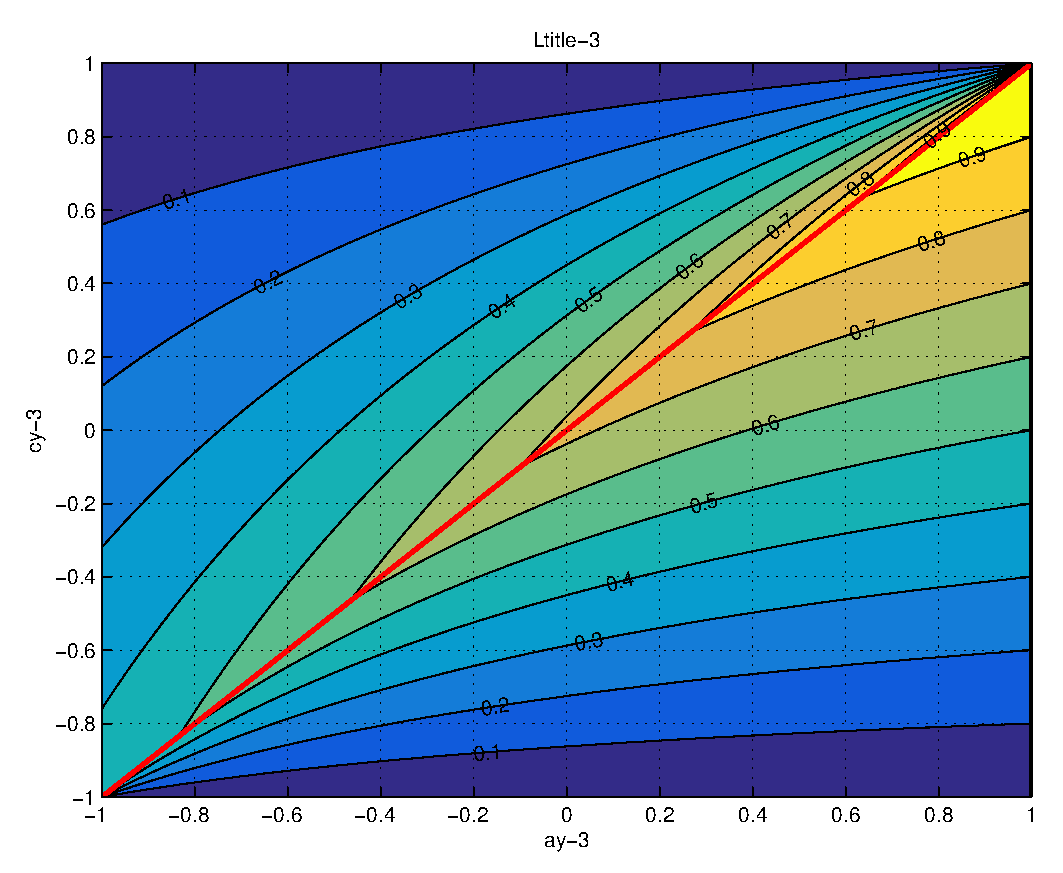
\includegraphics{img/espace_stat_max3.eps}}
\caption{}
\end{subfigure}

\begin{subfigure}[h]{0.8\textwidth}
\psfrag{-0.1}[cc][cc][1][0]{$0.1$}
\psfrag{-0.2}[cc][cc][1][0]{$0.2$}
\psfrag{-0.3}[cc][cc][1][0]{$0.3$}
\psfrag{-0.4}[cc][cc][1][0]{$0.4$}
\psfrag{-0.5}[cc][cc][1][0]{$0.5$}
\psfrag{-0.6}[cc][cc][1][0]{$0.6$}
\psfrag{-0.7}[cc][cc][1][0]{$0.7$}
\psfrag{-0.8}[cc][cc][1][0]{$0.8$}
\psfrag{-0.9}[cc][cc][1][0]{$0.9$}
\psfrag{-1}[cc][cc][1][0]{$-1$}
\psfrag{1}[cc][cc][1][0]{$1$}
\psfrag{0.1}[cc][cc][1][0]{$0.1$}
\psfrag{0.2}[cc][cc][1][0]{$0.2$}
\psfrag{0.3}[cc][cc][1][0]{$0.3$}
\psfrag{0.4}[cc][cc][1][0]{$0.4$}
\psfrag{0.5}[cc][cc][1][0]{$0.5$}
\psfrag{0.6}[cc][cc][1][0]{$0.6$}
\psfrag{0.7}[cc][cc][1][0]{$0.7$}
\psfrag{0.8}[cc][cc][1][0]{$0.8$}
\psfrag{0.9}[cc][cc][1][0]{$0.9$}
\psfrag{0}[cc][cc][1][0]{$0$}
\psfrag{cy-4}[cc][cc][1.2][0]{$c_y/\ell$ \ [m/m]}
\psfrag{ay-4}[cc][cc][1.2][0]{$a_y/\ell$ \ [m/m]}
\psfrag{Ltitle-4}[cc][cc][1.2][0]{$\mathcal{L}/(2L+\ell)$\ [m/m],\quad $\ell/L =1$}
\resizebox{1\textwidth}{!}{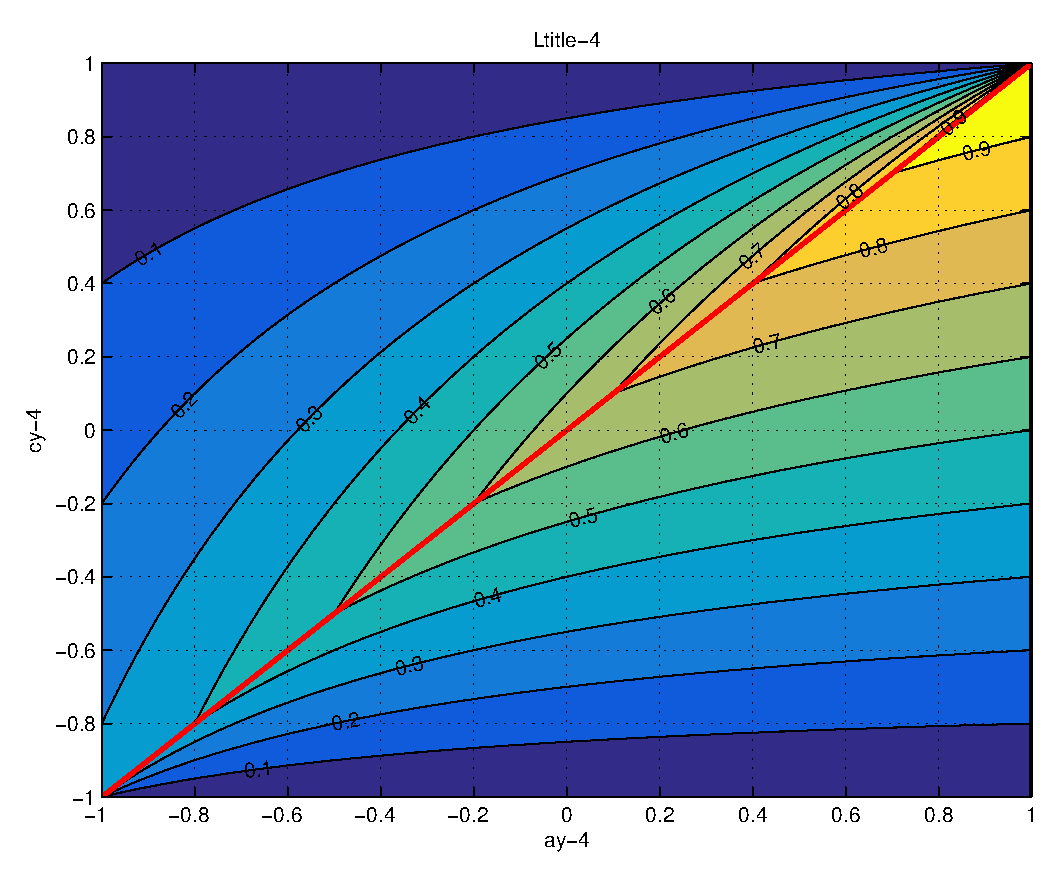
\includegraphics{img/espace_stat_max4.eps}}
\caption{}
\end{subfigure}
\caption[Variation de $\mathcal{L}$ en fonction de $a_y$ et $c_y$]{\label{chap1:fig:stat_max} Courbes de niveau de $\mathcal{L}$ en fonction des paramètres $a_y$ et $c_y$ et $\ell$.}
\end{figure} 
\clearpage
Dans chaque sous-figure de la figure \ref{chap1:fig:stat_max}, l’abscisse présente des valeurs de $a_y/\ell$ afin de mettre en évidence l'influence de la variation de $a_y$ dans la plage $]-\ell,\ell[$. Pour cette même raison, l'ordonné présente des valeurs de $c_y/\ell$. Les courbes de niveau sont obtenues en calculant le rapport $\mathcal{L}/(2L+\ell)$ à chaque couple ($a_y,c_y$) pour une valeur de $\ell$ donnée dans le titre de chaque sous-figure respective. le rapport de $\mathcal{L}/(2L+\ell)$ permet de normaliser la variation de $\mathcal{L}$ par rapport à sa valeur maximale et d'ainsi de mieux comprendre l'influence de $\ell$ sur la variation de $\mathcal{L}$.  La ligne rouge présente dans chaque sous-figure met en évidence les lieux dans le plan ($a_y,c_y$) où $a_y=c_y$. Les couples ($a_y,c_y$) qui respectent cette condition forme une crête sur laquelle $\mathcal{L}$ passe de 0 (la largeur de l'espace statique minimale) à $2L+\ell$ (la largeur maximale). Ces figures permettent de montrer qu'il est avantageux d'avoir des valeurs de $a_y$ et $c_y$ proche de $\ell$ afin d'obtenir la plus grande largeur possible de l'espace de travail statique. De plus, la présence de la ligne rouge permet de mettre en évidence le fait que la distance entre les courbes de niveau est plus importante en dessous qu'au dessus de la ligne $a_y=c_y$ lorsque $a_y$ et $c_y$ sont près de $\ell$ et qu'il est donc préférable d'avoir $c_y<a_y$ pour une valeur de $\mathcal{L}$ maximale. Une comparaison de la taille des sections jaunes dans les différentes figures montre qu'un faible rapport $\ell/L$ génère des valeurs de $\mathcal{L}$ plus importantes. Par conséquent, plus le rapport $\ell/L$ es faible, plus les valeurs de $a_y$ et $c_y$ doivent être proche de $\ell$ afin d'avoir une valeur de $\mathcal{L}$ importante.\par
Les premier point à retenir de l'analyse de l'espace de travail statique est que sa largeur est fonction des paramètres $a_y, c_y, \ell$ et $L$ d'après l'intervalle défini en (\ref{dom_stat}). De plus, Les limites de l'espace de travail statique sont définit comme les lieux dans le plan $XY$ où l'un des câbles du mécanisme voit sa tension tomber à zéro. La  largeur maximale de l'espace de travail statique est obtenue à l'aide de l'équation (\ref{chap1:eq:larg:stat}). Enfin, une analyse plus profonde de cette équation a permis de déterminer qu'il est préférable d'avoir le point $A_1$ et $C$ près du point $A_3$ afin d'avoir la largeur maximale de l'espace de travail statique et que cela est davantage . La section suivante porte sur l'application de forces externes sur l'effecteur.

\section{Application de forces externes}
Jusqu'à présent, aucune force ou moment externe n'ont été considérés dans la modélisation de la dynamique et dans l'étude de l'espace de travail statique. Or, certaines applications de robotique requièrent que le robot puisse supporter ou même appliquer des forces et des moments à son effecteur. Pour étudier l'application de forces et moments externes à l'effecteur du robot, cette section présente d'abord une analyse de l'équilibre statique du robot lorsqu'une force ou un moment est appliquée au centre de masse de l'effecteur. De cette analyse, une représentation géométrique de l'ensemble des torseurs d'actions pouvant être appliqués à l'effecteur est présentée. Enfin une optimisation de l'arrangement géométrique est proposé afin de maximiser généralement le torseur d'action pouvant être appliqué à l'effecteur.\par 
\subsection{Équilibre statique}
Afin de mieux comprendre l'influence des forces et des moments externes sur l'équilibre statique de l'effecteur, un torseur d'action externe $\mathbfcal{T}$ est appliqué au centre de masse de l'effecteur. La raison pour cette simplification est que tout ensemble de torseurs d'actions appliqué à différents points d'un corps peut inévitablement être représenté par une force et un moment autour du centre de masse du corps d'après la formule de Varignon. La figure suivante présente un diagramme de corps libre de l'effecteur lors de l'application du torseur d'action externe.
\begin{figure}[h!]
\centering
\psfrag{mg}[cc][cc][1][0]{\scriptsize$m\textbf{g}$}
\psfrag{Me}[cc][cc][1][0]{\scriptsize$M_e$}
\psfrag{te}[cc][cc][1][0]{\scriptsize$\mathbf{f}_e$}
\psfrag{f1}[cc][cc][1][0]{\scriptsize$-f_2\textbf{e}_2$}
\psfrag{f2}[cc][cc][1][0]{\scriptsize$-f_1\textbf{e}_1$}
\psfrag{f3}[cc][cc][1][0]{\scriptsize$-f_3\textbf{e}_2$}
\resizebox{0.5\textwidth}{!}{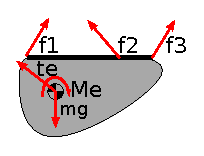
\includegraphics{img/equilibre_stat_ext.eps}}
\caption[DCL de l'effecteur avec forces externes]{\label{chap1:fig:equi_stat_ext}Diagramme de corps libre de l'effecteur lors de l'application d'un torseur d'action mécanique $\mathbfcal{T}=[\mathbf{f}_e,M_e]^T$ .}
\end{figure}
À la figure \ref{chap1:fig:equi_stat_ext}, $\mathbf{f}_e$ est la force externe appliquée au centre de masse de l'effecteur et $M_e$ est le moment externe appliqué au centre de masse de l'effecteur par unité de masse. L'équation suivante décrit l'équilibre statique de l'effecteur en tenant compte du torseur d'action externe appliqué au centre de masse 
\begin{align}
\mathbf{M}\bm{\tau}=\bm{\gamma}_e \label{chap1:eq:mat_n_e_ext},
\end{align}
où 
\begin{align}
\bm{\gamma}_e = \bm{\gamma}+\mathbfcal{T}=
\begin{bmatrix}
g+f_x \\ f_y \\ M_e
\end{bmatrix},\label{chap1:eq:gamma_e}
\end{align}
et où $\mathbf{M}$,$\bm{\tau}$ et $\bm{\gamma}$ sont les même matrice et vecteurs qu'à l'équation (\ref{mat_n_e}). À l'équation (\ref{chap1:eq:gamma_e}), $f_x$ et $f_y$ sont les composantes de forces de $\mathbf{f}_e$ selon l'axe $X$ et $Y$ du torseur d'action $\mathbfcal{T}$ par unité de masse. \par
\subsection{Représentation géométrique des torseurs possibles}
il est possible d'appliquer un torseur d'action $\mathbfcal{T}$ au centre de masse de l'effecteur si l'équation matricielle (\ref{chap1:eq:mat_n_e_ext}) admet une solution pour $\bm{\tau}\succ 0$ telle que $\bm{\tau}\succ 0$. Physiquement, cela veut dire que l'équilibre statique doit être maintenue tout en gardant les trois câbles tendus. Pour déterminer l'ensemble des torseurs qui respectent les conditions de tension, il est nécessaire de déterminer les torseurs qui mettent à zéro la tension dans l'un ou plusieurs câbles. La première étape pour déterminer ces torseurs limites consiste à évaluer l'équation (\ref{chap1:eq:mat_n_e_ext}) lorsque $f_i=0, i=1,2,3$. Cette valeur peut alors être enlevée du vecteur $\bm{\tau}$ ainsi que le $i$ème vecteur colonne de $\mathbf{M}$ ce qui donne le système suivant
\begin{align}
\mathbf{M}_{i[3\times 2]}\bm{\tau}_{i[2\times 1]} = \bm{\gamma}_{e},\quad i=1,2,3 \label{chap1:eq:eq_fx_i_dim}
\end{align}
où $\mathbf{M}_{i}$ est la matrice $\mathbf{M}$ avec la $i$ème colonne manquante, $\bm{\tau}_{i}$ est le vecteur $\bm{\tau}$ avec la $i$ème ligne manquante. S'il existe une solution à l'équation (\ref{chap1:eq:eq_fx_i_dim}), alors $\bm{\gamma}_{e}$ est une image de $\mathbf{M}_{i}$. Par conséquent, le déterminant de la matrice augmentée $\mathbf{M}_{a-i}$ définit comme 
\begin{align}
\mathbf{M}_{a-i} = \begin{bmatrix}
\mathbf{M}_{i} & |\bm{\gamma}_{e}
\end{bmatrix},
\end{align}
est nécessairement nul. En calculant le déterminant de chaque matrice augmentée, les égalisant à 0 et en manipulant les résultats obtenues, les trois équations suivantes sont obtenues
\begin{align}
\mathcal{P}_i:\left(A_i+B_iy\right)(f_x+g)+\left(C_i+B_ix\right)f_y+D_iM_e =0,\quad i=1,2,3, \label{chap1:eq:3_plans}
\end{align}
où 
\begin{align}
D_i=\frac{C_i}{c_x},\quad i=1,2,3.
\end{align}
Les trois équations en (\ref{chap1:eq:3_plans}) décrivent trois plans $\mathcal{P}_i$ dans l'espace des composantes de $\mathbfcal{T}$ et décrivent les limites des torseurs d'actions pouvant être appliqués à l'effecteur tout en maintenant son équilibre statique. L'orientation des trois plan est fonction de l'arrangement géométrique de l'effecteur ainsi que de sa position. La figure \ref{chap1:fig:torseur_poly} présente les trois plans pour un arrangement et une position de l'effecteur donnés dans le haut de la figure. 
\begin{figure}[h!]
\centering
\psfrag{004}[cc][cc][1.2][0]{$L =5$ m, $\ell=1 $ m, $a_y = 0$ m, $c_y = 0$ m, $c_x = 0$ m, $x = 5$ m, $y = 0$ m}
\psfrag{001}[cc][cc][1.2]{$f_y/g$}
\psfrag{002}[cc][cc][1.2]{$M_e/g$ [m]}
\psfrag{003}[cc][cc][1.2]{\rotatebox{180}
{$f_x/g$}}
\psfrag{005}[cc][cc][1.2]{$\mathcal{P}_1$}
\psfrag{006}[cc][cc][1.2]{$\mathcal{P}_1$}
\resizebox{0.8\textwidth}{!}
{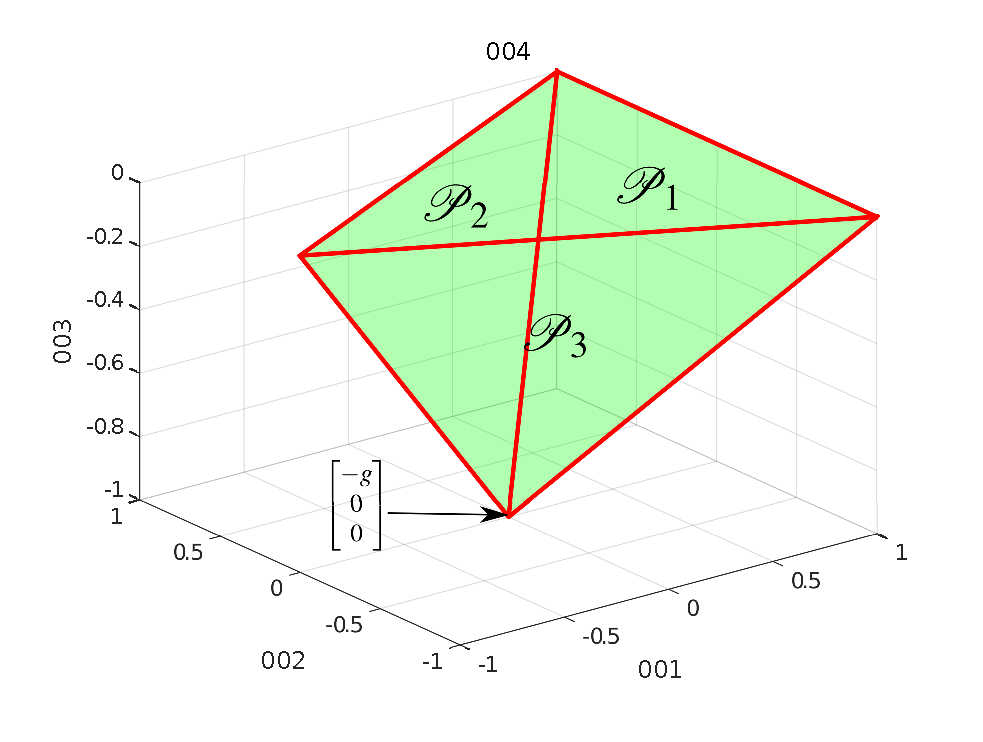
\includegraphics{img/torseur_poly.eps}}
\caption[Tétraèdre des torseurs]{\label{chap1:fig:torseur_poly}Intersections des plans $\mathcal{P}_i$ formant un tétraèdre dans l'espace des composantes du torseur $\mathbfcal{T}$.}
\end{figure}
Les trois plans et leurs intersections forment les trois côtés d'un tétraèdre inversée de hauteur infinie. Le sommet du tétraèdre est toujours situé au point au point $[-g,0,0]^T$ peut importe l'arrangement géométrique de l'effecteur. Cela peut facilement être vérifié en résolvant le système d'équation suivant
\begin{align}
\begin{bmatrix}
A_1+B_1y & C_1+B_1x & D_1 \\
A_2+B_2y & C_2+B_2x & D_2 \\
A_3+B_3y & C_3+B_3x & D_3
\end{bmatrix}
\mathbfcal{T}
= -g
\begin{bmatrix}
A_1+B_1y\\
A_2+B_2y\\
A_3+B_3y
\end{bmatrix}
\end{align} dont la solution est $\mathbfcal{T} = [-g, 0, 0]^T$. La signification physique de ce point d'intersection est que lorsqu'une force de $mg$ est appliquée au centre de masse de l'effecteur et dans la direction opposée à l'axe des $X$ (expliquant le signe négatif de la composante du torseur), l'effecteur devient alors automatiquement déséquilibré et il ne peut subir aucune autre moment ou force. Le fait que le tétraèdre ne possède pas de base signifie que plus la composante de force $f_x$ est grande, plus il est possible d'appliquer des composantes de forces latérales $f_y$ et de moments $M_e$ importants. \par
Afin de pouvoir déterminer l'influence des paramètres géométriques sur l'espace des torseurs d'action possible, un plan à $f_x=0$ est établie comme étant la base du tétraèdre. La hauteur du tétraèdre est alors de $g$ et le volume de celui-ci peut être utilisé comme un outil de mesure de l'espace des torseurs d'actions possible en fonction des paramètres géométriques de l'effecteur. La première étape afin de calculer le volume du tétraèdre consiste à calculer les vecteurs coïncident avec les arrêtes latérales du tétraèdre partant du sommet en $[-g, 0, 0]^T$ jusqu'au trois autres sommets à la hauteur $f_x=0$. La positions des sommets à $f_x=0$ peut être obtenue en solutionnant les systèmes d'équations suivants
\begin{align}
\begin{bmatrix}
C_i+B_ix & D_i \\
C_j+B_jx & D_j
\end{bmatrix}
\end{align}
% \subsubsection{Valeur maximale de $f_x$}
% Afin de déterminer la composante de force maximale selon l'axe $X$, $f_x$, le vecteur $\bm{\gamma}_e$ devient $\bm{\gamma}_{ex} = [g+f_x, 0,0]$. La valeur de $f_x$ maximale est ensuite obtenue en déterminant lequel des câbles du robot perd complètement sa tension pour la plus petite valeur de $f_x$. Mathématiquement, cela s'écrit \begin{align}
% f_x = \text{min}(f_x^1, f_x^2, f_x^3),
% \end{align}
% où $f_x^i$ est la composante de force minimale à appliquée au centre de masse de l'effecteur selon l'axe $X$ afin de faire perdre complètement sa tension au câble $i$. Pour calculer les $f_x^i$, la première étape consiste à évaluer l'équation (\ref{chap1:eq:mat_n_e_ext}) lorsque $f_i=0$. Cette valeur peut alors être enlevée du vecteur $\bm{\tau}$ ainsi que le $i$ème vecteur colonne de $\mathbf{M}$ ce qui donne le système suivant
% \begin{align}
% \mathbf{M}_{i[3\times 2]}\bm{\tau}_{i[2\times 1]} = \bm{\gamma}_{ex}^i,\quad i=1,2,3 \label{chap1:eq:eq_fx_i_dim}
% \end{align}
% où $\mathbf{M}_{i}$ est la matrice $\mathbf{M}$ avec la $i$ème colonne manquante, $\bm{\tau}_{i}$ est le vecteur $\bm{\tau}$ avec la $i$ème ligne manquante et $\bm{\gamma}_{ex}^i$ est le vecteur $\bm{\gamma}_{ex}$ avec $f_x$ remplacé par $f_x^i$. S'il existe une solution à l'équation (\ref{chap1:eq:eq_fx_i_dim}), alors $\bm{\gamma}_{ex}^i$ est une image de $\mathbf{M}_{i}$. Par conséquent, le déterminant de la matrice augmentée $\mathbf{M}_{a-i}$ définit comme 
% \begin{align}
% \mathbf{M}_{a-i} = \begin{bmatrix}
% \mathbf{M}_{i} & |\bm{\gamma}_{ex}^i
% \end{bmatrix},
% \end{align}
% est nécessairement nul. En calculant le déterminant de chaque matrice augmentée, les égalisant à 0 et en manipulant les résultats obtenues, les trois équations suivantes sont obtenues
% \begin{align}
% (A_i+B_iy)(g+f_x^i)=0,\quad i=1,2,3.\label{chap1:eq:sol_fx} 
% \end{align}
% Le premier zéro de l'équation (\ref{chap1:eq:sol_fx}) est identique aux équations sources de l'espace de travail statique en (\ref{chap1:ineq:ES1}) ce qui fait beaucoup de sens considérant que les bornes de l'espace de travail statique indique une position dans le plan $XY$ où la tension dans l'un des câbles est nulle. Le deuxième zéro de l'équation en (\ref{chap1:eq:sol_fx}) est également très intuitif. En effet, si la composante de force externe par unité de masse appliquée à l'effecteur est égale à $g$, alors les tensions dans les câbles sont nécessairement nulle puisque la force externe compense complètement pour le poids de l'effecteur. Comme ce deuxième zéro est le même pour les trois câbles, le développement précédent permet donc de prouver que la composante maximale de force par unité de masse pouvant être appliquée le long de l'axe des $X$ est de $g$ et pointant vers le haut ( dans le sens contraire de la gravité).
% \subsubsection{Valeur maximale de $f_y$}
% La même méthode que celle développée à la sous section précédente est utilisée pour déterminer la valeur maximale de $f_y$. Par conséquent, le vecteur $\bm{\gamma}_{e}$ devient $\bm{\gamma}_{ey}=[g,f_y,0]^T$. Les trois équations permettant de déterminer les $f_y^i$, obtenues en calculant le déterminant des matrices augmentées sont 
% \begin{align}
% f_y^i = \frac{-g(A_i+B_iy)}{C_i+B_ix},\quad i=1,2,3. \label{chap1:eq:tens_y_max}
% \end{align}
% Les différentes valeurs de $f_y^i$ peuvent avoir des signes différents. Or, pour que le robot soit versatile, il davantage pratique s'il peut appliquer des forces dans les deux directions. Pour cette raison, une nouvelle variable $\Delta f_y$ est ici définie comme la différence entre la composante maximale de force pouvant être appliquée dans la direction de l'axe $Y$ moins la composante de force maximale pouvant être appliquée dans la direction opposée à l'axe $Y$. Mathématiquement, l'expression pour $\Delta f_y$ est alors
% \begin{align}
% \Delta f_y = max^*(f_y^1, f_y^2, f_y^3)
% \end{align}
% \section{Planification de trajectoires dynamiques}
% Les équations scalaires en (\ref{cond_scal}) établissent les conditions qui doivent être satisfaites en tout point d'une trajectoire afin que l'ensemble des câbles du mécanisme soient sous tension. Cette section du mémoire utilise ces conditions afin de planifier des trajectoires elliptiques générales ainsi que les trajectoires de transition vers ces trajectoires elliptiques. L’attrait des trajectoires elliptiques est qu'elle peuvent représenter à la fois des lignes et des cercles en plus d'utiliser des combinaisons de fonctions trigonométriques, ce qui permet certaines simplifications. Cette section présente dans un premier temps la forme paramétrique d'une trajectoire paramétrique ainsi que ses dérivée. Ensuite, l'équation paramétrique et sa dérivée sont substitués dans les conditions générales établies en (\ref{cond_scal}) afin d'obtenir des conditions propres aux trajectoires elliptiques qui assureront que les câbles du mécanisme sont toujours sous tension. Enfin, des trajectoires de transition sont établies qui permettent de faire la transition du repos vers la trajectoire elliptique générale.
\subsection{Trajectoires elliptiques générales}
Une ellipse centrée au point $(x_c, y_c)$ dans un plan $XY$, ayant une longueur de grand rayon de $r_x$ et une longueur de petit rayon de $r_y$ et orientée avec un angle de $\theta$ par rapport à l’abscisse $X$  est représenté à la figure \ref{chap1:fig:ell_c} et son équation paramétrique temporelle s'écrit 
\begin{align}
\mathbf{p}_e(t) &= \begin{bmatrix}
x_e(t)\\y_e(t)
\end{bmatrix} = \mathbf{p}_c +  \mathbf{p}_d(t), \label{chap1:eq:gen_ell}\\
\mathbf{p}_c =\begin{bmatrix}
x_c \\ y_c
\end{bmatrix},\quad \mathbf{p}_d(t) &=
\begin{bmatrix}
r_x\cos(\theta)\cos(\omega t+\phi)-r_y\sin(\theta)\sin(\omega t+\phi)\\
r_x\sin(\theta)\cos(\omega t+\phi)+r_y\cos(\theta)\sin(\omega t+\phi)
\end{bmatrix}, \label{chap1:eq:ell_base}
\end{align}
où $t$ est le temps en seconde et $\omega$ est ici appelée la fréquence d'oscillation et décrit combien de fois par seconde (s) un tour complet (oscillation) autour de l’ellipse est effectué par un point suivant la trajectoire $\mathbf{p}_e(t)$ en rad/s. Conséquemment, la période de cette trajectoire est de $T = \frac{2\pi}{\omega}$ s. La valeur $\phi$ est en radians et  permet d'établir la position initiale de la trajectoire sur l'ellipse. Puisque le vecteur $\mathbf{p}_d(t)$ et ses composantes sont utilisés à plusieurs reprises dans les sections suivantes, $\mathbf{p}_d(t)$ est simplifié sous la forme \begin{align}
\mathbf{p}_d(t) = r_y\begin{bmatrix}
\sin(\omega t+\phi_x)\\
\sin(\omega t+\phi_y)
\end{bmatrix} 
\label{chap1:eq:gen_ell_simp}
\end{align}
où $\phi_x$ et $\phi_y$ sont ici appelées les phases elliptiques et s'écrivent
\begin{align}
\phi_x = \tan^{-1}\left(\frac{\sin(\theta)\sin(\phi)-k\cos(\theta)\cos(\phi)}{k\cos(\theta)\sin(\phi)+\sin(\theta)\cos(\phi)}\right)\\
\phi_y = \tan^{-1}\left(\frac{k\sin(\theta)\cos(\phi)+\cos(\theta)\sin(\phi)}{\cos(\theta)\cos(\phi)-k\sin(\theta)\sin(\phi)}\right)
\end{align}
et où $k$ est le rapport entre $r_x$ et $r_y$ tel que 
\begin{align}
k =\frac{r_x}{r_y}
\end{align}

La forme paramétrique en (\ref{chap1:eq:ell_base}) est particulièrement intéressante car elle permet de produire des trajectoires linéaires et circulaires en établissant différentes valeurs au paramètres de l'équation. Le développement associé à la formulation de trajectoire linéaires et circulaires à l'aide de l'équation générale elliptique est présenté à l'annexe C. \par 
la dérivée et la double dérivée par rapport au temps de la trajectoire en (\ref{chap1:eq:gen_ell_simp}) donnent respectivement la  vitesse et l'accélération de la trajectoire en fonction du temps. Les dérivés se calculent
\begin{align}
\dot{\mathbf{p}}_e(t) = \frac{d}{dt}\mathbf{p}_e(t) = r_y\omega \begin{bmatrix}
\cos(\omega t + \phi_x)\\
\cos(\omega t + \phi_y)
\end{bmatrix}
\\
\ddot{\mathbf{p}}_e(t) = \frac{d^2}{dt^2}\mathbf{p}_e(t) = -r_y\omega^2 \begin{bmatrix}
\sin(\omega t + \phi_x)\\
\sin(\omega t + \phi_y)
\end{bmatrix} \label{chap1:eq:accel_ell}
\end{align}
où $\dot{\mathbf{p}}_e(t)$ et $\ddot{\mathbf{p}}_e(t)$ sont respectivement les vecteurs de vitesse et d'accélération de la trajectoire.\par 
La sous-section suivante présente la substitution des équations (\ref{chap1:eq:gen_ell_simp}) et (\ref{chap1:eq:accel_ell}) dans les conditions scalaires en (\ref{cond_scal}) pour déterminer des conditions propres aux trajectoires elliptiques qui assure la tension dans les câbles. 
\subsection{Substitutions dans les conditions de tension}
Les conditions permettant d'assurer la tension dans les câbles du mécanisme lors de trajectoires elliptiques générales sont obtenues en substituant les expressions (\ref{chap1:eq:gen_ell_simp}) et (\ref{chap1:eq:accel_ell}) dans les conditions générales de tension en (\ref{cond_scal}). En manipulant les résultats de la substitutions à l'aide d'identités trigonométriques, les résultats suivants sont obtenues
\begin{align}
h_i(t)<0,\quad i=1,2,3
\label{chap1:eq:cond_scal_ell}
\end{align}
où 
\begin{align}
h_i(t) = r_y\left(\Delta_{1i}\sin(\omega t)+\Delta_{2i}\cos(\omega t)\right)+g\Psi_i, i=1,2,3.
\label{chap1:eq:cond_scal_ell_hi}
\end{align}
où 
\begin{align*}
\Delta_{1i} &= k\Phi_i  \cos(\phi_x) + \Upsilon_i  \cos(\phi_y)\\
\Delta_{2i} &= k\Phi_i  \sin(\phi_x) + \Upsilon_i  \sin(\phi_y)\\
\Phi_i &= \omega^2\Psi_i\\
\Upsilon_i &= gB_i-\omega^2\Omega_i\\
\Psi_i &= A_i + B_iy_c\\
\Omega_i &=C_i+B_ix_c.\label{eq:k}
\end{align*}
Toutes les fonctions en (\ref{chap1:eq:cond_scal_ell}) sont des fonctions périodiques. Par conséquent, une preuve suffisante que les câbles sont sous tension à tous moments pendant une trajectoire elliptique est de montrer que toutes les valeurs extrêmes des $h_i(t)$ sont inférieures à 0, c'est à dire que toutes les conditions en (\ref{chap1:eq:cond_scal_ell}) sont respectées lorsque les fonctions périodiques sont évaluées à leurs extrêmes. Les extrêmes des $h_i(t)$ peuvent être trouvés en calculant la dérivée temporelle des $h_i(t)$ et en mettant égale à zéro les résultats, ce qui donne
\begin{align}
\frac{d h_i(t)}{d t} = r_y\omega\left(\Delta_{1i} \cos(\omega t) - \Delta_{2i} \sin(\omega t)\right) = 0 \quad i = 1,2,3.
\end{align}
Les extrêmes des fonctions trigonométriques sont alors trouvés en solutionnant les équations suivantes \begin{align}
\Delta_{1i} \cos(\omega t) = \Delta_{2i} \sin(\omega t), i=1,2,3.
\end{align}
Pour résoudre ces équations, l'identité trigonométrique $\cos^2(x)+\sin^2(x)=1$ est utilisé ce qui donne les solutions suivantes
\begin{align}
\cos(\omega t) &=\pm \frac{\Delta_{2i}}{\Theta_i},\quad \sin(\omega t) =\pm \frac{\Delta_{1i}}{\Theta_i}, \quad i =1,2,3. \label{eq: trig_simp}
\end{align}
où
\begin{align*}
    \Theta_i = \sqrt{\Delta_{1i}^2+\Delta_{2i}^2 }.
\end{align*}
En substituant les valeurs en (\ref{eq: trig_simp}) dans les conditions en (\ref{chap1:eq:cond_scal_ell_hi}), 4 fois 3 pour un total de 12 conditions sont obtenues qui doivent être satisfaites afin d'assurer la tension des les câbles du robot lors d'une trajectoire elliptique générale. Ces conditions prennent la forme 
\begin{align}
    \frac{r_y\left(\pm \Delta_{1i}^2 \pm \Delta_{2i}^2\right)}{\Theta_i}+g\Psi_i < 0, \quad i =1,2,3, \label{eq:cond_no_time}
\end{align}
où les 4 conditions pour chaque câble ($i$) sont analogues au 4 combinaisons différentes possible des deux $\pm$. Les conditions en (\ref{eq:cond_no_time}) sont toutes indépendantes du temps et permettent ainsi  de mettre directement en relation l'amplitude d'oscillation $r_y$ et la fréquence d'oscillation $\omega$. Effectivement, pour chaque $i$ il est possible d'isoler $r_y$ dans les conditions en (\ref{eq:cond_no_time}) pour obtenir des relations qui limitent l'amplitude d'oscillation. Ces conditions s'écrivent
\begin{align}
    r_y &> \frac{g\Psi_i \Theta_i }{\Delta_{1i}^2 + \Delta_{2i}^2} \label{eq: ineq_ell_1}\\
    r_y &< \frac{-g\Psi_i \Theta_i}{\left|\Delta_{2i}^2 - \Delta_{1i}^2\right|}\label{eq: ineq_ell_23}\\
    r_y &< \frac{-g\Psi_i \Theta_i}{\Delta_{1i}^2 + \Delta_{2i}^2}, i =1,2,3 \label{eq: ineq_ell_4}
\end{align}
où la condition en (\ref{eq: ineq_ell_23}) satisfait à la fois les conditions avec $\left(+\Delta_{1i}^2 - \Delta_{2i}^2\right)$ et $\left(- \Delta_{1i}^2 + \Delta_{2i}^2\right)$ en (\ref{eq:cond_no_time}). Il est possible de diminuer le nombre de conditions à respecter  en déterminant si l'un des groupes de conditions assure le respect des deux autres. Par inspection, $r_y$ est nécessairement une valeur positive réelle car elle représente la grandeur du petit rayon de la trajectoire elliptique. $\Delta_{1i}^2$ et $\Delta_{2i}^2$ sont deux valeurs positives puisque elles représentes respectivement des valeurs élevées au carré. Enfin, $g$ est une valeur positive et $\Theta_i$ est nécessairement une valeur positive car elle représente un terme en racine carrée et doit être réelle afin que $r_y$ puisse être réelle. Cette inspection porte à la conclusion que $\Psi_i$ doit nécessairement être négatif et que par conséquent, le seul respect de la  condition (\ref{eq: ineq_ell_4}) assure le respect des deux autres conditions. En effet, si $\Psi_i$ est positif, alors aucun des trois groupe de condition en (\ref{eq: ineq_ell_1}), (\ref{eq: ineq_ell_23}) et (\ref{eq: ineq_ell_4}) ne peuvent être respectée simultanément. Or, si la valeur de $\Psi_i$ est plus petite que 0, toute les conditions peuvent être respectées en même temps. Puisque $\Psi_i$ doit être négatif, les conditions en (\ref{eq: ineq_ell_1}) deviennent inutiles car elles sont toutes respectées si $r_y>0$. Enfin, puisque $\Delta_{1i}^2$ + $\Delta_{2i}^2$ est toujours plus grand que $\left|\Delta_{2i}^2 - \Delta_{1i}^2\right|$, le respect des conditions en (\ref{eq: ineq_ell_4}) assure le respect des conditions en  (\ref{eq: ineq_ell_23}). Le respect des conditions en (\ref{eq: ineq_ell_4}) assure donc le respect de toutes les autres conditions. \par
Un fait important mentionné dans le paragraphe précédent est que $\Psi_i<0$ est nécessaire afin de pouvoir assurer la tension dans les câbles du mécanisme lors d'une trajectoire elliptique. L'interprétation physique de cette condition mathématique est que la position en $Y$ du centre de l'ellipse doit se trouver à l'intérieur de l'espace statique de travail. Il s'agit d'une condition importante qui concorde avec des articles similaires (Mettre le num des articles similaires ici.) portant sur des trajectoires elliptiques en 3D.\par
Les conditions en (\ref{eq: ineq_ell_4}) peut être simplifiées sous la forme 
\begin{align}
 r_y < \frac{-g\Psi_i}{\sqrt{k^2\Phi_i^2 + \Upsilon_i^2 + 2k\Phi_i\Upsilon_i\cos(\eta)}}, i = 1,2,3,\label{eq:ineq_simp}
\end{align}
où 
\begin{align}
\eta = \phi_x-\phi_y = \tan^{-1}\left(\frac{k}{(k^2-1)\cos(\theta)\sin(\theta)}\right).\label{chap1:eq:eta}
\end{align}
La simplification en (\ref{eq:ineq_simp}), montre que les conditions assurant la tension dans les câbles du mécanisme sont indépendantes de la position initiale sur l'ellipse de la trajectoire qui est donnée par le terme $\phi$.
\begin{comment}
\section{Rigidité du mécanisme}
La rigidité d'un robot est typiquement associé à sa matrice de rigidité qui met en relation le déplacement de son effecteur avec un torseur d'action de forces appliqués à l'effecteur sous la forme
\begin{align}
\mathbf{F} = \mathbf{K}\bm{\Delta} \mathbf{x},
\end{align}
où $\mathbf{F} = [f_x, f_y, M_\phi]^T$ est le torseur d'action de forces appliquées à l'effecteur, $\bm{\Delta} \mathbf{x}= [\Delta x, \Delta y, \Delta \phi]^T$ est un vecteur représentant des déplacements en translation et en rotation et $\mathbf{K}$ est la matrice de rigidité qui est calculée à l'aide de la matrice $\mathbf{M}$ de l'équation (\ref{M}) comme 
\begin{align}
\mathbf{K}=k\mathbf{MM}^T,
\end{align}
où $k$ est la rigidité des actionneurs qui sont habituellement modélisés comme des ressorts linéaires. Dans le cas où les membres sont des barres ou des des poutres, la rigidité est typiquement modélisée comme étant la même en tension et en compression. Cependant, dans le cas des câbles, la rigidité devient plutôt une quantité qui dépend de la direction de la force passant dans celui-ci puisque les câbles ne supportent pas les forces de compression. Mathématiquement, la rigidité d'un câble, $k_c$, peut être modélisé comme 
\begin{align}
k_c = \begin{cases}
\frac{k_Ik_m}{k_I+k_m}, \quad&f >0
\\0, \quad &f\leq0
\end{cases},
\end{align}
où $k_I$ est la rigidité intrinsèque du câble qui est fonction de son module d'élasticité, de sa longueur et de son diamètre, $k_m$ est le raideur du moteur actionnant le câble et $f$ est la force passant dans le câble telle qu'une force positive signifie une force de tension. La condition $f>0$ pour le câble $i$ du mécanisme a été précédemment étudié à la section 1.5 comme étant satisfaite statiquement si la condition (\ref{chap1:ineq:ES1}) était respectée. Or, cette condition ne considère pas l'application de forces externes à l'effecteur.
\end{comment}
\begin{comment}
$\mathcal{L}$ est donc, entre autre, fonction des paramètres $a_y$ et $c_y$. Puisque l'équation (\ref{chap1:eq:larg:stat}) contient la fonction max(), il est difficile de déterminer analytiquement quelles valeurs de $a_y$ et $c_y$ produisent la largeur de l'espace statique de travail la plus importante. Par simple inspection de la figure \ref{fig:chap1:geometrie}, il pourrait sembler intuitif que la largeur maximale de l'espace statique soit de $2L$, soit du point $B_1$ jusqu'au point milieu entre les points $B_2$ et $B_3$. Or, la valeur maximale de $\mathcal{L}$ est en réalité de $2L+\ell$. Ce maximum advient lorsque $a_y=c_y=\ell$. Dans cette situation, le mécanisme devient équivalent à un mécanisme à masse ponctuelle à deux câbles ( les câbles 1 et 3) comme celui présenté dans les articles [mettre les articles ici]. La figure \ref{chap1:fig:compare_pm} présente le mécanisme lorsque $a_y=c_y=\ell$ en mettant en évidence le fait que, dans cette configuration géométrique, le mécanisme est équivalent au mécanisme à masse ponctuelle des articles [mettre article ici]. Bien qu'il soit avantageux dans plusieurs situations d'avoir un espace de travail statique le plus large possible, Lorsque $a_y=c_y=\ell$, le mécanisme perd sa propriété de garder constante l'orientation de l'effecteur puisque le câble 2 ne perçoit plus de tension. Par conséquent, cette disposition géométrique est à éviter afin de permettre au mécanisme de garder constante son orientation. 
\begin{figure}[h!]
\centering
\resizebox{0.75\textwidth}{!}{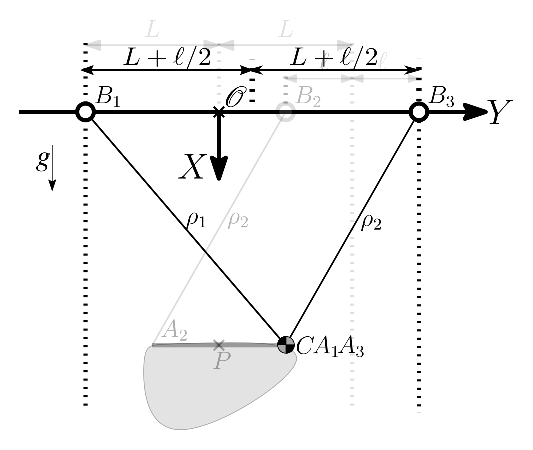
\includegraphics{img/geo_base_comp_pm.eps}}
\caption{\label{chap1:fig:compare_pm} Disposition géométrique maximisant la largeur de l'espace de travail statique.}
\end{figure}
\\
Afin de déterminer quelles combinaisons de $a_y$ et $c_y$ maximisent l'espace de travail statique tout en gardant l'orientation de l'effecteur constante, un script MATLAB est utilisé afin de tester plusieurs combinaisons possibles de $a_y$ et $c_y$. Le pseudo-code du script prend la forme suivante
\begin{lstlisting}
% discrétisation de ay et cy sur 100 points dans l'interval -l à l
ay = linspace(-l,l,100);
cy = linspace(-l,l,100);
% Boucle sur l'ensemble des combinaisons
for i =1:length(ay)
    B2   = aya(i)-l;
    B3   = -(aya(i)+l);
    for j =1:length(cy)
        A3 = ay(i)*(L-cy(j))-2*L*cy(j)-l*(ay(i)+L);
        A2 = ay(i)*(cy(j)-L)+2*L*cy(j)-l*(ay(i)+L);
        Larg(i,j) = L - max(-A3/B3,-A2/B2);
    end
end
\end{lstlisting}
où \mcode{Larg} est la matrice contenant toutes les valeurs de $\mathcal{L}$. La figure \ref{chap1:fig:stat_max} présente la variation de $\mathcal{L}$ en fonction des paramètres $a_y$ et $c_y$ issue du script précédent.
\begin{figure}[h!]
\begin{center}
\psfrag{-0.1}[cc][cc][1][0]{$0.1$}
\psfrag{-0.2}[cc][cc][1][0]{$0.2$}
\psfrag{-0.3}[cc][cc][1][0]{$0.3$}
\psfrag{-0.4}[cc][cc][1][0]{$0.4$}
\psfrag{-0.5}[cc][cc][1][0]{$0.5$}
\psfrag{-0.6}[cc][cc][1][0]{$0.6$}
\psfrag{-0.7}[cc][cc][1][0]{$0.7$}
\psfrag{-0.8}[cc][cc][1][0]{$0.8$}
\psfrag{-0.9}[cc][cc][1][0]{$0.9$}
\psfrag{-1}[cc][cc][1][0]{$-1$}
\psfrag{1}[cc][cc][1][0]{$1$}
\psfrag{0.1}[cc][cc][1][0]{$0.1$}
\psfrag{0.2}[cc][cc][1][0]{$0.2$}
\psfrag{0.3}[cc][cc][1][0]{$0.3$}
\psfrag{0.4}[cc][cc][1][0]{$0.4$}
\psfrag{0.5}[cc][cc][1][0]{$0.5$}
\psfrag{0.6}[cc][cc][1][0]{$0.6$}
\psfrag{0.7}[cc][cc][1][0]{$0.7$}
\psfrag{0.8}[cc][cc][1][0]{$0.8$}
\psfrag{0.9}[cc][cc][1][0]{$0.9$}
\psfrag{0}[cc][cc][1][0]{$0$}
\psfrag{cy}[cc][cc][1][0]{$c_y/\ell$ \ [m/m]}
\psfrag{ay}[cc][cc][1][0]{$a_y/\ell$ \ [m/m]}
\psfrag{annot}[cc][cc][1][0]{$a_y=c_y$}
\psfrag{Ltitle}[cc][cc][1][0]{$\mathcal{L}/2L$\ [m/m]}
\resizebox{0.75\textwidth}{!}{\includegraphics{img/espace_stat_max.eps}}
\caption{\label{chap1:fig:stat_max} Largeur de $\mathcal{L}$ en fonction de $a_y$ et $c_y$.}
\end{center}
\end{figure}
Les valeurs dans l'abscisse et l'ordonné sont divisée par la valeur $\ell$ afin d'obtenir des valeurs relatives à la largeur de l'effecteur et puisque, comme mentionné précédemment, $a_y$ doit être contenu dans l'intervalle $]-\ell,\ell[$. Les valeurs des courbes de niveau représentes le rapport de $\mathcal{L}$ sur $2L$ afin de montrer quels couples $(a_y,c_y)$ produisent une largeur $\mathcal{L}$ supérieure à l'espace de travail maximal intuitif. La ligne rouge désigne l'ensemble des couples 
$(a_y,c_y)$ où $a_y=c_y$. C'est sur cette ligne que se situe les couples $(a_y,c_y)$ qui maximise l'espace de travail statique. En effet, la courbe de niveau dans le coin supérieur droit de la figure \ref{chap1:fig:stat_max} indique une valeur supérieure à 1 sans être à $a_y =\ell$. Cependant, la largeur de l'espace statique n'est pas le seul critère de performance statique du mécanisme. Afin de mieux identifier le choix optimal du couple $(a_y, c_y)$, la sous-section suivante présente une analyse de la rigidité statique du mécanisme.
\subsubsection{Rigidité en translation et en rotation}
La rigidité du mécanisme est divisée en deux sous catégories, la rigidité en translation et la rigidité en rotation. La rigidité en translation est ici définie comme la force minimale à appliquer au centre de masse de l'effecteur afin de le faire bouger en translation le long de l'axe $Y$. La composante de force à appliquer le long de l'axe $X$ est toujours $-mg$ puisque le mécanisme est suspendu et par conséquent, l'étude de la rigidité dans cette direction n'est pas pertinente. Une méthode possible afin de déterminer la force de minimale permettant la translation de l'effecteur selon l'axe $Y$ est de remplacer une à une les tension dans chaque câble par une force parallèle à l'axe des $Y$, de calculer la nouvelle matrice de Newton-Euler, d'inverser cette matrice et de multiplier la matrice inverse par le vecteur $\bm{\gamma}$ présenté à l'équation (\ref{mat_n_e}). Mathématiquement, cela s'écrit
\begin{align}
\begin{bmatrix}
f_i\\f_j\\\tau_{yij}
\end{bmatrix} = \begin{bmatrix}
\begin{bmatrix}\mathbf{e}_i &\mathbf{e}_j \\
\delta_i & \delta_j\end{bmatrix}\begin{bmatrix}
0 \\ 0 \\ 1
\end{bmatrix}
\end{bmatrix}^{-1}\begin{bmatrix}g\\ 0\\ 0 \end{bmatrix}, (i,j) = \binom{3}{2},
\label{chap1:eq:stiff_lat}
\end{align}
o\`u $\tau_{yij}$ est la force lattérale à appliquer pour maintenir l'équilibre statique du mécanisme lorsque seulement les câbles $i$ et $j$ sont conservés (ne sont pas remplacés). En gardant la dernière ligne de chaque équation matricielle en (\ref{chap1:eq:stiff_lat}), les trois équations suivantes sont obtenues
\begin{align}
\tau_{y23} &= \frac{-g(A_1 + B_1y)}{C_1+B_1x} \\
\tau_{y13} &= \frac{-g(A_2 + B_2y)}{C_2+B_2x} \\
\tau_{y12} &= \frac{-g(A_3 + B_3y)}{C_3+B_3x}.
\end{align}
où les $A_i$, $B_i$ et $C_i$ sont présentés à l'équation (\ref{cond_scal}). Des trois valeurs de $\tau_{yij}$ obtenues dans les équations précédentes, celle dont la valeur absolue est a plus proche de 0 définie la rigidité en translation du mécanisme, ici nommée $\tau_y$. Mathématiquement, $\tau_y$ est obtenue par l'expression suivante
\begin{align}
\tau_y = \text{min}\left(\abs{\tau_{y23}}, \abs{\tau_{y13}}, \abs{\tau_{y12}}\right),
\end{align}
où min() est une fonction qui retourne la valeur minimale de ses arguments.
\end{comment}












